%%%%%%%%%%%%%%%%%%%%%%%%%%%%%%%%%%%%%%%%%%%%%%%%%%%%%%%%%%%%%%%%%%%%%%%%%%%%
% AGUJournalTemplate.tex: this template file is for articles formatted with LaTeX
%
% This file includes commands and instructions
% given in the order necessary to produce a final output that will
% satisfy AGU requirements, including customized APA reference formatting.
%
% You may copy this file and give it your
% article name, and enter your text.
%
%
% Step 1: Set the \documentclass
%
%

%% To submit your paper:
\documentclass[draft]{agujournal2019}
\usepackage{url} %this package should fix any errors with URLs in refs.
\usepackage{lineno}
\usepackage[inline]{trackchanges} %for better track changes. finalnew option will compile document with changes incorporated.
\usepackage{soul}
\usepackage{amsmath}
\usepackage{siunitx}
\usepackage{color}
\newcommand{\red}[1]{\textcolor{red}{#1}}
\newcommand{\blue}[1]{\textcolor{blue}{#1}}

\linenumbers
%%%%%%%
% As of 2018 we recommend use of the TrackChanges package to mark revisions.
% The trackchanges package adds five new LaTeX commands:
%
%  \note[editor]{The note}
%  \annote[editor]{Text to annotate}{The note}
%  \add[editor]{Text to add}
%  \remove[editor]{Text to remove}
%  \change[editor]{Text to remove}{Text to add}
%
% complete documentation is here: http://trackchanges.sourceforge.net/
%%%%%%%

\draftfalse

%% Enter journal name below.
%% Choose from this list of Journals:
%
% JGR: Atmospheres
% JGR: Biogeosciences
% JGR: Earth Surface
% JGR: Oceans
% JGR: Planets
% JGR: Solid Earth
% JGR: Space Physics
% Global Biogeochemical Cycles
% Geophysical Research Letters
% Paleoceanography and Paleoclimatology
% Radio Science
% Reviews of Geophysics
% Tectonics
% Space Weather
% Water Resources Research
% Geochemistry, Geophysics, Geosystems
% Journal of Advances in Modeling Earth Systems (JAMES)
% Earth's Future
% Earth and Space Science
% Geohealth
%
% ie, \journalname{Water Resources Research}

\journalname{JGR: Oceans}


\begin{document}

%% ------------------------------------------------------------------------ %%
%  Title
%
% (A title should be specific, informative, and brief. Use
% abbreviations only if they are defined in the abstract. Titles that
% start with general keywords then specific terms are optimized in
% searches)
%
%% ------------------------------------------------------------------------ %%



\title{Melt response to calving events in Pine Island Glacier}

%% ------------------------------------------------------------------------ %%
%
%  AUTHORS AND AFFILIATIONS
%
%% ------------------------------------------------------------------------ %%

% Authors are individuals who have significantly contributed to the
% research and preparation of the article. Group authors are allowed, if
% each author in the group is separately identified in an appendix.)

% List authors by first name or initial followed by last name and
% separated by commas. Use \affil{} to number affiliations, and
% \thanks{} for author notes.
% Additional author notes should be indicated with \thanks{} (for
% example, for current addresses).

% Example: \authors{A. B. Author\affil{1}\thanks{Current address, Antartica}, B. C. Author\affil{2,3}, and D. E.
% Author\affil{3,4}\thanks{Also funded by Monsanto.}}

\authors{A. T. Bradley\affil{1}, D. Bett\affil{1}, P. Dutrieux\affil{1}, J. De Rydt\affil{2}, P. Holland\affil{1}}


% \affiliation{1}{First Affiliation}
% \affiliation{2}{Second Affiliation}
% \affiliation{3}{Third Affiliation}
% \affiliation{4}{Fourth Affiliation}

\affiliation{1}{British Antarctic Survey, High Cross, Madingley Road, Cambridge CB3 0ET, UK}
\affiliation{2}{Department of Geography and Environmental Sciences, Northumbria University, Newcastle upon Tyne, UK.}

%(repeat as many times as is necessary)

%% Corresponding Author:
% Corresponding author mailing address and e-mail address:

% (include name and email addresses of the corresponding author.  More
% than one corresponding author is allowed in this LaTeX file and for
% publication; but only one corresponding author is allowed in our
% editorial system.)

% Example: \correspondingauthor{First and Last Name}{email@address.edu}

\correspondingauthor{Alexander Bradley}{aleey@bas.ac.uk}

%% Keypoints, final entry on title page.

%  List up to three key points (at least one is required)
%  Key Points summarize the main points and conclusions of the article
%  Each must be 100 characters or less with no special characters or punctuation and must be complete sentences

% Example:
% \begin{keypoints}
% \item	List up to three key points (at least one is required)
% \item	Key Points summarize the main points and conclusions of the article
% \item	Each must be 100 characters or less with no special characters or punctuation and must be complete sentences
% \end{keypoints}

%\begin{keypoints}
%\item 
%\item
%\item  
%\end{keypoints}

%% ------------------------------------------------------------------------ %%
%
%  ABSTRACT and PLAIN LANGUAGE SUMMARY
%
% A good Abstract will begin with a short description of the problem
% being addressed, briefly describe the new data or analyses, then
% briefly states the main conclusion(s) and how they are supported and
% uncertainties.

% The Plain Language Summary should be written for a broad audience,
% including journalists and the science-interested public, that will not have 
% a background in your field.
%
% A Plain Language Summary is required in GRL, JGR: Planets, JGR: Biogeosciences,
% JGR: Oceans, G-Cubed, Reviews of Geophysics, and JAMES.
% see http://sharingscience.agu.org/creating-plain-language-summary/)
%
%% ------------------------------------------------------------------------ %%
\newcommand{\mpryr}{~m~yr\textsuperscript{-1}}


%% \begin{abstract} starts the second page

\begin{abstract}
[ enter your Abstract here ]
\end{abstract}

\section*{Plain Language Summary}
[ enter your Plain Language Summary here or delete this section]


%% ------------------------------------------------------------------------ %%
%
%  TEXT
%
%% ------------------------------------------------------------------------ %%
\section{Introduction}\label{S:Introduction}
%we have seen big changes, and they're mostly driven by increased basal melting

Ice sheets and ice shelves in West Antarctica have undergone significant changes in recent years, characterized by an increasing rate of ice loss~\cite{Paolo2015Science}, glacier acceleration, and grounding line retreat. For Pine Island Glacier, which sits in this region, these changes have been particularly acute: Pine Island has experienced a 70\% increase in ice flux and a close to doubling of surface velocity between 1974 and 2013~\cite{Mouginot2014GRL}, while its grounding line retreated some 31~km at its centre between 1992 and 2011~\cite{Rignot2014GRL}. Increased basal melting has been implicated as a key driver of these changes~\cite{Pritchard2012Nature, Rignot2019PNAS}: ice shelves offer a resistive stress (commonly referred to as `buttressing') that restrains the flow of grounded ice; increased basal melting reduces ice shelf volume and thus the buttressing they are able to provide~\cite{Gudmundsson2013Cryo, Reese2018NatureClimCh, Gudmundsson2019GRL,Gagliardini2010GRL,Goldberg2019GRL}.

%depth of the pycnocline is the most important factor
The main source of heat for ice shelf melting in the Amundsen Sea off West Antarctica is Circumpolar Deep Water (CDW), which sits below lighter Winter Water. In the Amundsen Sea, the pycncocline that separates these two water masses remains mostly above the level of the continental shelf break~\cite{Heywood2016Oceanography}, allowing a significant amount of CDW, and thus heat, to spill onto the continental shelf and reach ice shelf cavities. The depth of the pycnocline is not constant, but varies significantly on decadal timescales~\cite{Jenkins2018NatureGeo}; years with a deeper pycnocline tend to result in lower meltwater fluxes from ice shelves, and vice versa.

\begin{figure}
    \centering
    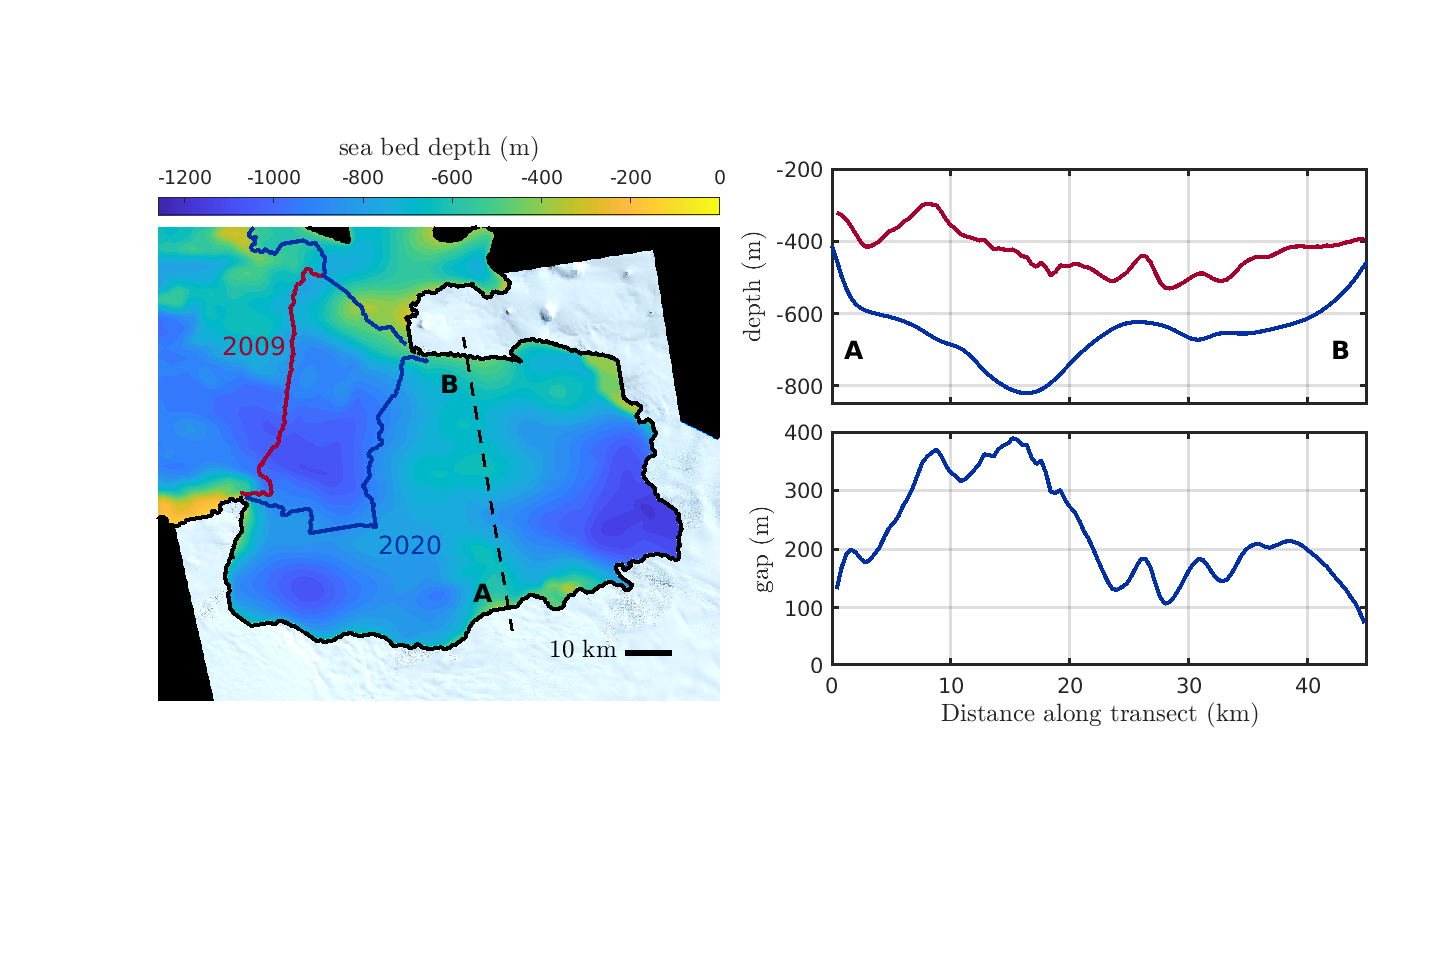
\includegraphics[width = \textwidth]{../make_figures/plots/figure1.eps}
    \caption{(a) Contour plot of seabed depth under Pine Island ice shelf and in Pine Island pay (colours) alongside the location of the ice front in 2009 (red line) and 2020 (blue line). The solid black line indicates the grounding line from \cite{Joughin2010GRL}, and the background image is a Sentinel 2 mosaic from November 2020. The black dashed line indicates the approximate location of the crest of the seabed ridge. (b) Seabed bathymetry (blue) and ice draft (red) taken along the dashed line in (a). (c) Plot of the ridge-seabed gap measured along the dashed black line in (a) (i.e. the difference between the red and blue lines in (b)). \red{Remove whitespace and also add co-ordinate lines?}}
    \label{fig:figure1}
\end{figure}


%ridge in PIG makes pycnocline picture more complicated
For Pine Island, this simple `pycnocline depth' picture is complicated by the presence of a seabed ridge in the ice shelf cavity. This ridge is located several tens of kilometers upstream of the grounding line, and protrudes several hundred metres above the seabed (figure~\ref{fig:figure1}). In combination with the ice shelf directly above it, the ridge acts as a topographic barrier that restricts the access of CDW to an inner cavity that has formed between the ridge and the grounding line since the ice shelf grounding line likely retreated from this ridge in the late 1940s~\cite{Jenkins2010NatureGeo, DeRydt2014JGeophysResOceans, DeRydt2016JGeophysResEarthSurf}. The particular geometry of the cavity means that the strength of the topographic barrier (i.e. how much its presence affects sub-shelf melting) is strong dependent on the pycncoline depth: at its shallowest, the pycnocline sits above the depth of the ridge crest, and a large amount of modified CDW is able to spill into the inner cavity~\cite{Dutrieux2014Science}; in contrast, at its lowest, the pycnocline sits some way below the ridge crest and CDW access is severely restricted.  As a result, melting of Pine Island Glacier has a particularly strong sensitivity to hydrographic conditions in Pine Island Bay: Dutrieux et al. reported that the total freshwater flux from the fast flowing part of Pine Island Glacier in 2009 (80~km\textsuperscript{3}~year\textsuperscript{-1}), when the pycnocline was at its second highest level on record, was more than double its value in 2012 (37~km\textsuperscript{3}~year\textsuperscript{-1}), when the pyncocline was at the second lowest recorded depth.

%another thing we have seen is significant calving events
In addition to it's unique topographic control on melting, the recent calving of Pine Island Ice Shelf also stands out amongst Amundsen Sea terminating ice shelves. Mass losses from ice sheets in Antarctica are dominated by calving and melting~\cite{Rignot2013Science}; in equilibrium, these losses must balance the upstream accumulation of ice. The recent retreat of the Pine Island ice shelf (PIIS) front, however, suggests that the calving rate is far higher than would be required to maintain an equilibrium; the ice front retreated approximately 26km between 2009 to 2020 (figure~\ref{fig:figure1}), with the majority of this retreat happening over 2015--2020~\cite{Lhermitte2020PNAS, Joughin2021ScienceAdv}. These changes correspond to a more-than-doubling of the calving rate, from approximately 4~km~year\textsuperscript{-1} to approximately 9~km~year\textsuperscript{-1}.

%at present, the ridge is located approx x km downstream of the ridge crest. The changes some far have been implicated in a speed up because of a loss of buttressing, but might the changes have also led to a relaxation of the topographic barrier and thus and increase in melt rates (that would only be evidenced on longer timescales(?)) [key question one]
As of 2020, the ice front is located approximately 20~km downstream of the ridge (figure~\ref{fig:figure1}), and the ice front is now closer to the ridge crest that the location of the ice front prior to 2015. The loss of buttressing associated with this retreat has been shown to be responsible for the significant speed up of PIG since 2015~\cite{Joughin2021ScienceAdv}. However, given that the topographic barrier to CDW relies on the combination of ice draft \textit{and} seabed ridge, the recent calving events beg the following question: have recent calving events relaxed the topographic barrier, leading to significant changes in melting in PIIS?

%but also, in future, we might have further calving events because or preconditioning and or MICI that might bring to ridge to the crest. How might these potential future calving events lead to changes in melt rates? [key question two]
Here, in addition to addressing the effect on melt rates of calving events that have already happened, we also consider changes that might result from future calving events. It has been suggested that damage to the ice shelf has preconditioned PIIS to calving further in the future~\cite{Lhermitte2020PNAS} and that if calving presents a higher ice cliff to the ocean, that may trigger runaway calving events (the so called marine ice cliff instability~\cite{DeConto2016Nature}). Both of these mechanisms may lead to significant calving in the future; the second main question we aim to answer in this paper is: how might these potential future calving events lead to changes in melt rates?

In this paper, we use numerical simulations in both idealized and realistic geometries to assess how, and why, melt rates in PIIS will respond to past and potential future calving events. We begin in \S\ref{S:Experiment} with a description of the idealized experiments, setting out details of the ocean model used and the experimental setup. We perform a total of nine idealized experiments; results of one such experiment (the `baseline') are presented in \S\ref{S:Baseline}: we describe how and why the melt rate responds to calving in this baseline experiment. In the following two sections, we discuss how the picture presented in \S\ref{S:Baseline} changes for different cavity geometries (\S\ref{S:Results:H}) and hydrographic forcings (\S~\ref{S:Results:P}). In \S\ref{S:Realistic}, we describe and present results from experiments that uses a geometry that closely matches real world conditions for PIIS. Guided by the results of the idealized experiments, we assess the response of melt rates to calving events. Finally, in \S\ref{S:Discussion}, we discuss the results of this experiment in the realistic geometry and in \S\ref{S:Summary}, we summarize our findings.

%what we're going to do: use a combination of idealized and real world modelling to attempt to answer these questions. 

%in this paper, we explore the response of melting to calving in an idealized setup. We aim to isolate the physical processes responsible. Idealized modelling also means that 
%In this paper, we aim to 



%\begin{figure}
%    \centering
%    \includegraphics{}
%    \caption{Info on realistic PIG}
%    \label{fig:figure1}
%\end{figure}

\section{Experiment Details}\label{S:Experiment}
%broad overview of the experiemnts
We perform a total of nine experiments in idealized geometries, each corresponding to a unique pair of parameters that characterize the variable ice shelf cavity geometry and hydrographic forcing (described in sections \S\ref{S:Experiment:Geometry} and \S\ref{S:Experiment:Hydrography}, respectively). Each experiment consists of a series of ten simulations in which the ice front position is systematically varied, thus simulating calving; each simulation involved explicitly resolving the ocean circulation using the MIT general circulation model (MITgcm). Other than removing sections of the ice shelf, the ice shelf geometry does not change within each experiment. Ice shelves themselves enter the simulations passively, via the exchange of heat and salt at the ice-ocean interface alone (i.e. there are no ice-dynamics considerations in the cavity geometry); a passive description of ice shelves is sufficient to assess the response of melt rates to ice shelf calving, which occur on timescales much shorter than on which the ice responds dynamically to perturbations in melting. In the following sections we provide further details of the ocean model and experimental setup, including the motivation for various parameter choices.
\begin{figure}
    \centering
    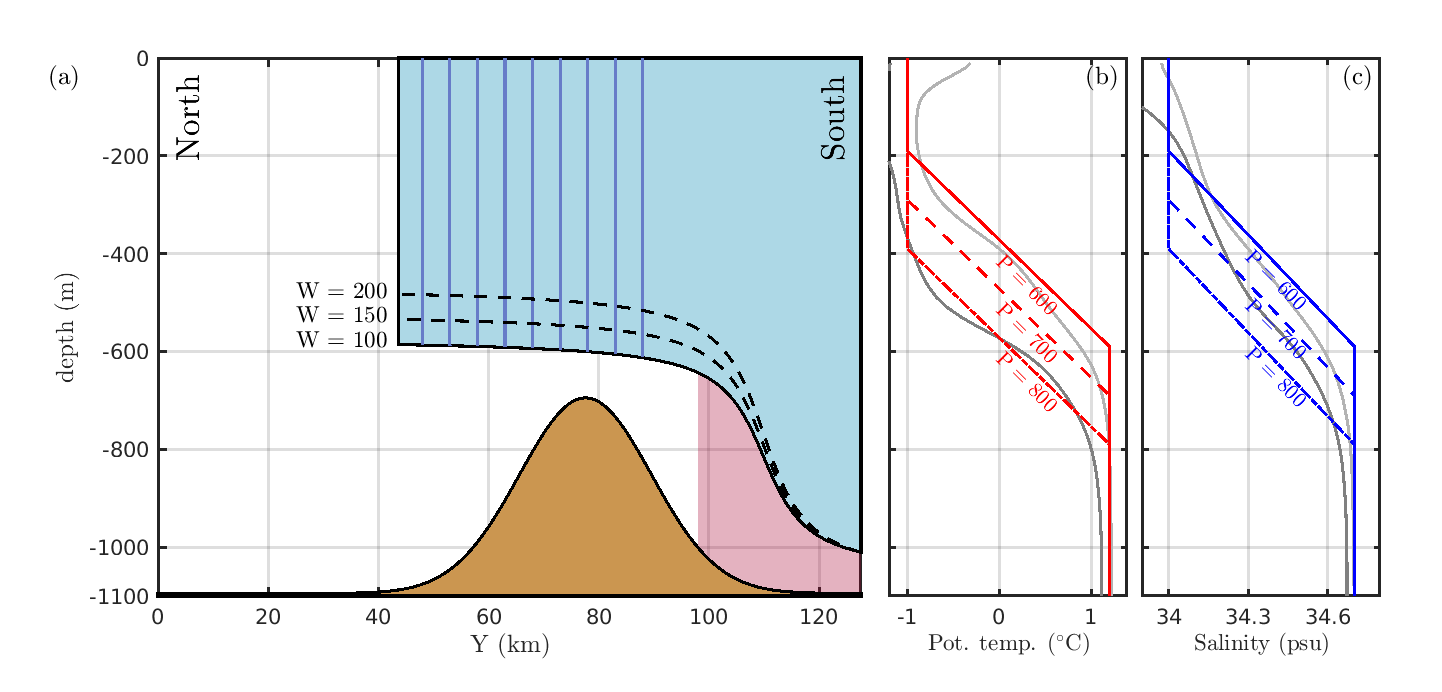
\includegraphics[width = \textwidth]{../make_figures/plots/figure2.eps}
    \caption{(a) Schematic diagram of the experimental setup. The domain is uniform in the third (into the page) dimension, with extent 48~km. The ocean domain consists of the gridded area, which is bordered by a passive ice shelf (shaded blue) and seabed ridge a (shaded brown). Solid and dashed black lines indicate the ice shelf geometry used in the default simulation for the three values of the ridge-gap parameter $W$=100~m, $W$=150~m, and $W$=200~m, as labelled. Solid blue lines indicate the ice front in the calving experiments, which are located 80, 75, 70, 65, 60, 55, 50, 45, and 40~km north of the southern end of the domain. The shaded red region indicates the inner cavity (see main text), defined as those locations in the ocean domain that are within 30~km of the southern end of the domain. (b) Salinity and temperature profiles used in the experiments (red and blue curves), with $P$ = 600~m (solid), $P$ = 700~m (dashed), $P$ = 800~m (dot-dashed) as indicated by the label. Grey lines correspond to temperature and salinity profiles taken from CTD measurements in Pine Island Bay during the austral summers of 2009 (light grey) and 2012 (dark grey).}
    \label{fig:figure2}
\end{figure}

\subsection{Details of Ocean Model}\label{S:Experiment:Model}
The MITgcm is a z-level general circulation model that includes a partial-cell treatment of topography, allowing an accurate description of both the seabed and ice draft. Our model grid consists of 110 layers with a vertical spacing of 10~m, and a horizontal resolution of 400m. We use the MITgcm in hydrostatic mode with a implicit nonlinear free surface scheme, a third-order direct space-time flux limited advection scheme, a non-linear equation of state~\citeA{Mcdougall2003JAtmosOceanTech}, and the Pacanowski-Philander~\cite{Pacanowski1981JPhysOcean} scheme parametrizes vertical mixing. Constant values of 15 and 2.5~m\textsuperscript{2}~s\textsuperscript{-1} are used for the horizontal Laplacian viscosity and horizontal diffusivity. The equations are solved on an $f$-plane with $f = -1.4\times10^{-4}~\text{s}^{-1}$.

Each simulation is ran for at least 7 months, using a timestep of 30~\si{seconds}, after which time the configuration reaches a steady state. The melt rates reach approximately 95\% of their final values with three months. All results presented here are averaged over the final two months of the simulation. 

The MITgcm includes a static representation of ice shelves~\cite{Losch2008JGeophysResOceans}. Ice shelf melting is implemented using the so-called "three-equation formulation"~\cite{Holland1999JPhysOcean} that describes the exchange of heat and salt across the ice-ocean boundary. The implementation of this scheme in MITgcm has been described in detail elsewhere~\cite[for example]{DeRydt2014JGeophysResOceans,Dansereau2014JGROceans} but we note that thermal exchange across the ice-ocean interface is typically dominated by latent heat (a consequence of the fact that the temperature difference between ice shelves and the adjacent boundary layer is on the order of several degrees Celsius, while the characteristic temperature associated with latent heat removal is -84 degrees Celsius). With latent heat dominated thermal exchange, the three equation formulation simplifies to give the melt rate $\dot{m}$ as
\begin{equation}\label{E:MeltRate}
    \dot{m} = \frac{c_p \gamma_T (T - T_b)}{L}.
\end{equation}
Here $c_p = 3947~\si{\joule \kilogram}^{-1}$ is the specific heat capacity of water, $T$ is the temperature of the ocean side of a viscous boundary layer at the ice-ocean interface, $T_b$ is the temperature at the ice shelf base, which must be at the local freezing point, and $\gamma_T$ is a heat exchange co-efficient that parametrizes exchange across the boundary layer. The heat exchange coefficient has a weakly non-linear relationship on $u^*$, the ocean speed adjacent to the ice shelf base~\cite{Holland1999JPhysOcean}; assuming a perfectly linear relationship, equation~\eqref{E:MeltRateUdT} yields
\begin{equation}\label{E:MeltRateUdT}
    \dot{m} \propto u^* (T - T_b).
\end{equation}
We shall return to equation~\eqref{E:MeltRateUdT} when diagnosing the mechanisms responsible for melt rate variation with ice shelf calving.

All parameter values used in the three equation formulation here are as in~\citeA{Holland1999JPhysOcean}, with the exception of the drag co-efficient, which is set to $4.5\times10^{-3}$, a value that is more appropriate for Pine Island Glacier~\cite{Dutrieux2014Science} (the drag coefficient that enters in the momentum balance, which can be set independently, remains at the default value of $2.5\times 10^{-3}$).

\subsection{Ice Shelf Geometry and Seabed Bathymetry}\label{S:Experiment:Geometry}
Our idealized setup is shown schematically in figure~\ref{fig:figure2}a: it is uniform in the zonal direction, along which the $x$-axis is aligned, and the $y$-axis is aligned along the meridional direction (although PIG is aligned approximately East-West, we assume here that it is aligned East-West, as is standard~\cite{Grosfeld1997JGROceans, DeRydt2014JGeophysResOceans}).

The sea bed has a Gaussian profile,
\begin{equation}\label{E:Experiment:Bed}
    b(x,y) = -1100 + 400 \exp\left[-\frac{\left(y - 50\times 10^3\right)^2}{2\sigma^2}\right],
\end{equation}
where $\sigma = 12$~km is the length scale over which this profile decays towards zero. The profile~\eqref{E:Experiment:Bed} corresponds to a ridge that peaks 50km from the grounding line at the southern end of the domain, at a height of 400m (note that the cavity thickness is prevented from reaching zero at the grounding line as the MITgcm requires at least two grid cells in the vertical to permit horizontal transfer). 

The variability in both PIIS draft and the height of the seabed ridge result in a ridge-draft gap that varies between approximately 100m at its narrowest to greater than 300m at its widest (figure~\ref{fig:figure1}b,c). Since we assumed a constant sea bed geometry, we aim to capture the effect of variability in the ridge-draft gap by considering different values of $H$, the vertical distance between the crest of the seabed ridge and the ice shelf base; $H$ enters only the model only via the ice profile, which, following~\citeA{DeRydt2014JGeophysResOceans}, takes the form
\begin{equation}
    h(y) = \begin{cases}
    \left(\frac{310 + W}{2.64}\right)\tan^{-1}\left(\frac{y}{5882} -3\right) & \text{for}~y < y_f,\\
    0  & \text{for}~y \geq y_f.
    \end{cases}
\end{equation}
Here $y_f$ is the variable location of the ice front (see below). We stress that these ice profiles are not obtained from ice dynamics considerations, but do feature a flatter section beyond the ridge and a steeper section inside the ridge that is observed in practice (figure~\ref{fig:figure2}a).

We use three different values of $W$: $W$=100~m, $W$=150~m, and $W$=200m. The smallest value, $W = 100$m, corresponds to the minimum gap between the ice shelf and ridge that is observed in Pine Island (figure~\ref{fig:figure1}b,c), while the largest value, $W$=200m, corresponds to an upper bound, beyond which the melt response to calving is negligible, as we shall see. 

Within each experiment, the vary the front position $y_f$ is systematically reduced, essentially removing sections of ice and thus simulating calving. The ten simulations within each experiment use values $y_f$ = 84, 80, 75, 70, 65, 60, 55, 50, 45, and 40~km, which correspond to calved lengths of $l_c$= 0, 4, 9, 14, 19, 24, 29, 34, 39, and 44~km, respectively. The simulation with $y_f$ = 84~km is referred to as the default run within each experiment, serving as a benchmark against which results are compared. There are both pragmatic and physical reasons for choosing this particular range of values for $y_f$: the default experiment corresponds roughly to the distance of the ice front in PIG in 2009, before significant calving took place in the late 2010s; the lowest value, $y_f$ = 40~km, is chosen as a compromise between significant calving beyond the ridge, whilst retaining a large area that is shared by each experiment: as we discuss further in \S\ref{S:Baseline}, the area over which melt rates are averaged must be invariant to calving for a robust assessment of changes to melt rates with calving. The computational expense of ocean simulations together with a large number of experiments means that the number of simulations within the range is restricted to ten.

\subsection{Hydrographic Forcing}\label{S:Experiment:Hydrography}

As discussed in \S\ref{S:Introduction}, the presence of a seabed ridge in Pine Island Glacier means that melt rates are particularly sensitive to the depth of the pycnocline far from the ice shelf (the hydrographic forcing); we therefore expect that the melting response to calving will also have a sensitive dependence on hydrographic forcing. To assess this sensitivity, we perform each experiment with a different value of the ridge-gap parameter $W$ three times, each with a different hydrographic forcing. The hydrographic forcing is  imposed on the model by means of a restoring boundary condition at the northern end of the domain (figure~\ref{fig:figure2}): at this boundary, the temperature and salinity are restored to specified vertical profiles (see below) over a distance of five horizontal grid cells (total length 2km) with a restoring timescale that varies from 12~h at the boundary to 60~h at the interior of this restoring regions. (The model includes solid walls with a free slip condition at the southern, western, and eastern sides of the domain.)

%what do our profiles look like
The three temperature and salinity profiles to which the ocean is restored are shown in figure~\ref{fig:figure2}b,c. Both the temperature and salinity profiles are piecewise linear functions of depth, featuring a constant temperature and salinity in both an upper ($-1~\si{\celcius}$, salinity $34$~psu) and lower layer ($1.2~\si{\celcius}$, salinity $34.7$~psu), which separated by a pycnocline of thickness 400~m. The pycnocline begins at a variable depth $P$ (a higher $P$ corresponds to a deeper pycnocline), which parametrizes the whole profile; our three hydrographic forcings use $P = 600$, $700$, and $800$. 

%why do we choose these conditions
These piecewise linear profiles are approximations to typical conditions for the Pine Island Bay~\cite{Jacobs1996GRL, Dutrieux2014Science, Jenkins2018NatureGeo} (see figure~\ref{fig:figure2}a,b); the upper and lower layers are dominated by Winter Water and (modified) Circumpolar Deep Water, respectively. As mentioned, the record of hydrographic conditions in the Amundsen Sea points to significant variability in the depth of the pycnocline varies considerably on interannual timescales~\cite{Dutrieux2014Science}; the profiles with $P = 600$ and $P = 800$ correspond to the years 2009 and 2012, respectively, which span the range of observed conditions: in 2012, the average depth of the pycnocline was at the lowest on record, while in 2009, the average depth of the pycnocline was at the highest on record. 

%wrap up the experiments:\ 
The nine experiments are uniquely identified by a $(H,P)$ pair, where $H$ $\in \{100, 150, 200\}$ and $P$ $\in \{600, 700, 800\}$. We consider the extreme scenario with the strongest topographic barrier and warmest hydrographic forcing, $(H,P) = (100,600)$ to be the baseline; in the following section, we describe the results of this baseline experiment, before describing in sections~\ref{S:Results:H} and~\ref{S:Results:P} how this picture changes for different values of $H$ and $P$, respectively.

\section{Result for the Baseline Experiment ($H$=100~m, $P$=600~m)}\label{S:Baseline}
In this section, we describe the results for the baseline experiment with $W$ = 100~m and $P$ = 600~m, which correspond to the profiles with solid lines in figures~\ref{fig:figure2}a--c. We begin by describing the steady state configuration for the default (uncalved) simulation in this experiment, and then describe how, and why, calving changes the melt rate.

\subsection{Default Run}\label{S:Baseline:Default}
\begin{figure}
    \centering
    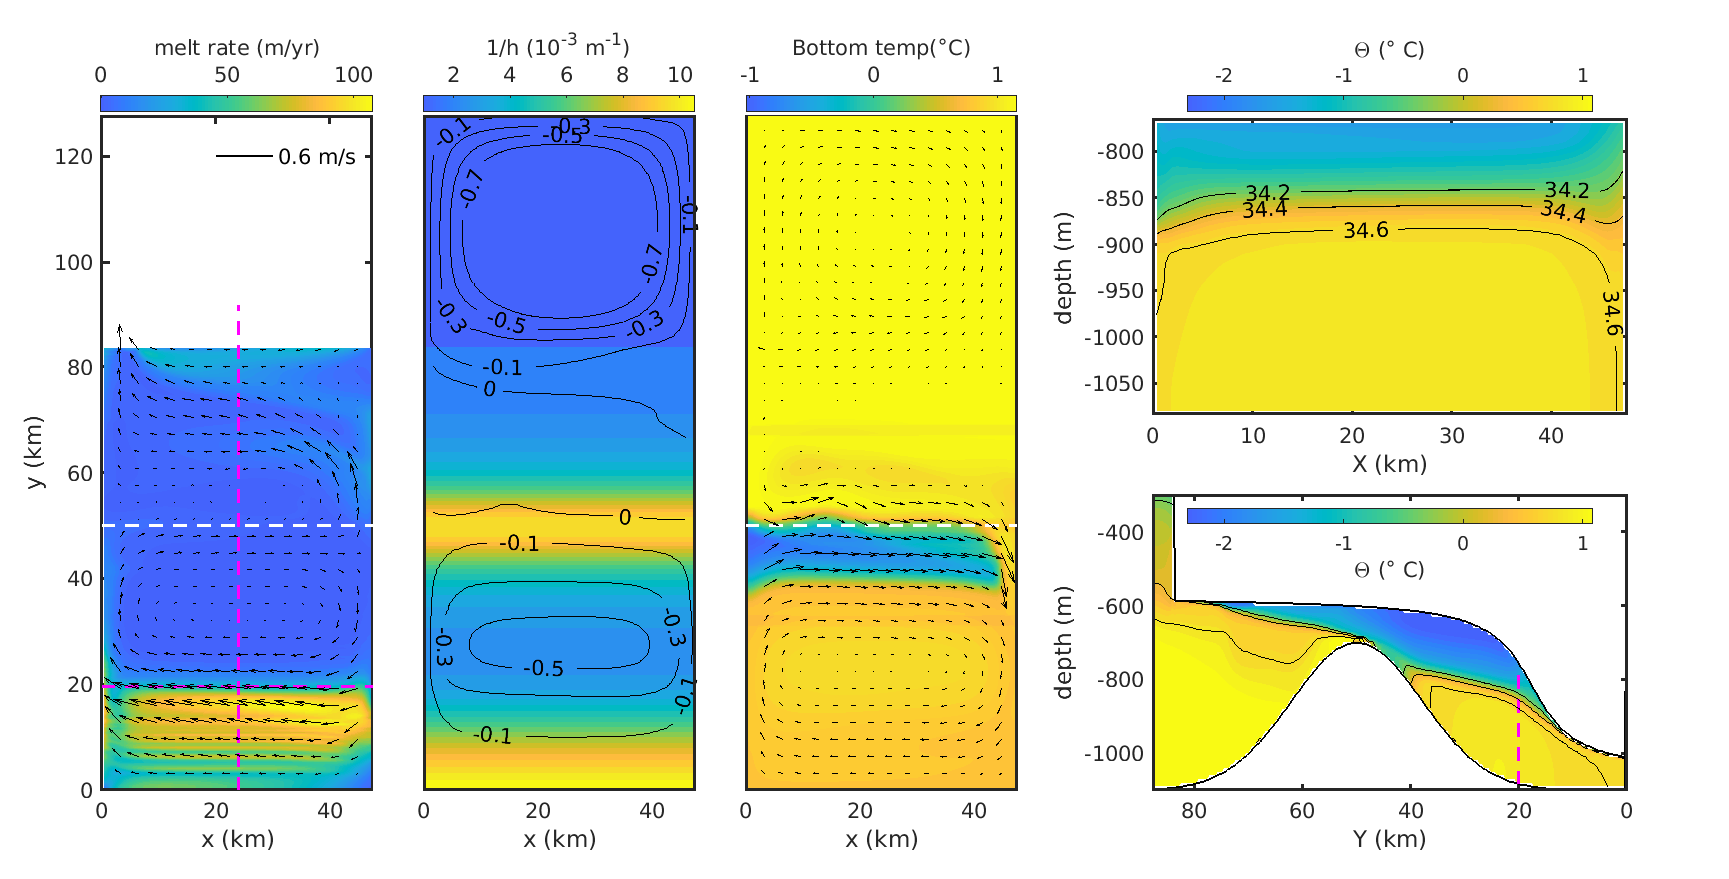
\includegraphics[width = \textwidth]{../make_figures/plots/figure3.eps}
    \caption{Ice-ocean properties that characterize the default (uncalved) simulation in the baseline experiment ($W$ = 100~m, $P$ = 600~m). (a) Melt rate (colours) and boundary layer velocities (arrows), averaged over the three grid cells adjacent to the ice-ocean interface. White areas correspond to open ocean. Every fifth boundary layer velocity is plotted. The black line indicates an arrow length that would correspond to 0.6~m~s\textsuperscript{-1}. The white dashed line indicates the location of the top of the ridge, where the section in (d) is taken. The profile in (e) is taken along the dashed magenta centreline. (b) Inverse water column thickness $1/h$ (colours) and barotropic stream function (black contours, in units of Sv). (c) Bottom temperature (colours) and bottom current (arrows) averaged over the three grid cells closest to the seabed. The scale bar in (a) is also appropriate for (c). (d) Zonal cross-section taken along the white dashed line in (a), showing potential temperature (colours) and salinity contours at the 34.2, 34.4, and 34.6~psu levels. (e) Meridional cross-section, taken along the magnenta dashed line in (a), with colours and contours as in (d).}
    \label{fig:figure3}
\end{figure}

%describe each of what we see: melt rate, general observations
Ice-ocean properties that characterise the default simulation are shown in figure~\ref{fig:figure3}. Melt rates (figure~\ref{fig:figure3}a) are below  20\mpryr everywhere, except for a region located within 20~km of the grounding line, where maximum melt rates of reach a maximum of approximately 120\mpryr. The average melt rate over the whole shelf is approximately 20\mpryr; this is lower than the estimated value of 33$\pm$2 based on observations in Pine Island Bay in 2009~\cite{Jenkins2010NatureGeo} (to which the $P=600$ case corresponds), as is to be expected given that the topographic barrier is stronger in this simulation that expected in practice (this simulation applies the smallest gap that is observed in practice \textit{anywhere} on the ridge, over the whole of the ridge).

%introduce the idea of the inner cavity, why do we use this metric
At this point, we introduce the definition on the `inner cavity': the area of the ocean that is located within 30~km of the Southern end of the domain (indicated by the red shaded region in figure~\ref{fig:figure2}a). We use the mean melt rate in the inner cavity as a single metric to quantify changes in melt rate with calving, and refer to this quantity henceforth as the `inner cavity melt rate'. It is necessary to consider the same area in each simulation because the melt rate is highly spatially variable (figure~\ref{fig:figure3}a); integrating over the whole shelf, for example, would make smaller shelves appear to have anomalously large melt rates since the region of high melt close to the grounding line would occupy a great proportion of the total shelf. %A spatially invariant area over which the melt rate is integrated is necessary because the melt rate under the ice shelf is highly spatially variable (figure~\ref{fig:figure3}a); for example, if we removed sections of ice in the default run \textit{without} changing the melt rate pattern, those runs with less ice (i.e. significant calving) would display larger mean melt rates over the whole shelf because the highest melt rates are concentrated near the grounding line.
The choice of 30~km for the length of the inner cavity region reflects a compromise between permitting calving a significant distance beyond the ridge (the smallest shelf we consider must be larger than the inner cavity region), while including a reasonably large section of the ice shelf over which the melt rate is averaged. Crucially, this choice of inner cavity includes the grounding line; changes in melt rate at the grounding line are particularly important for the dynamics of the ice sheet~\cite{Seroussi2014Cryo, Athern2017GRL}. Although the values of inner cavity melt rate \textit{are} dependent on the choice of cavity, we verified that the trends and key results of the following sections are independent of the choice of inner cavity, provided that it is taken sufficiently far from the maximal extent of any of the simulations; for the choice of 30~km, the inner cavity melt rate in the default run is 46\mpryr (see $l_c = 0$ data point in figure~\ref{fig:figure3}a).

%why does the melt rate look like it does
Melt rates depend strongly on the cavity circulation and thermal driving (see equation~\eqref{E:MeltRate}). Cavity circulation (figure~\ref{fig:figure3}a,c) is charaterized by a cyclonic circulation which is Coriolis-driven;  this circulation is directed northward and southward at the Eastern and Western boundaries ($x=$0~km and $x=$48~km), respectively. In the inner cavity, South of $y = 30$~km, the circulation is vigorous, but high melt rates are restricted to $y<$ 20~km: North of $y$=20~km, a cold, fresh, and thus buoyant, meltwater plume sits adjacent to the ice-ocean interface (figure~\ref{fig:figure3}e), rather than the modified warm water that is adjacent to the ice-ocean interface for $y < $ 20~km  (figure~\ref{fig:figure3}d); the thermal driving, and thus melt rates, are significantly lower North of $y$=20~km.


%we can use the bsf 
To understand this pattern of melt rates, it is instructive to consider the barotropic stream function (figure~\ref{fig:figure3}b). In general, if the circulation is geostrophic, with buoyancy driving force balancing Coriolis forces, the flow will be barotropic and flow will align with contours of constant $f/h$, where $h$ is the water column thickness and $f =$ -1.4$\times$10\textsuperscript{-4}~s\textsuperscript{-1} is the Coriolis parameter at 75${}^\circ$S; in these simulations, contours of constant water column thickness correspond to lines of constant $y$, aligned East-West. There are two main potential vorticity (PV) barriers; where the water column thickness changes rapidly and thus diverting the flow: the first is at the ice front, where the resulting divergent currents, and associated high velocities, lead to locally enhanced melt rates of up to 50\mpryr (figure~\ref{fig:figure2}a). The second is at the seabed ridge; as flow approaches the ridge, it is diverted Westward (figure~\ref{fig:figure2}a) to retain a constant potential vorticity. Ultimately, this PV barrier is sufficiently strong that little flow is able to penetrate across the ridge (note the 0 barotropic contour at the top of the ridge in figure~\ref{fig:figure3}b). The exception to this is a strong boundary current at the East, where flow divergence and relative vorticity permit flow perpendicular to contours of constant column this thickness which is Southward (Northward) in the East (West). The result of the strong PV barrier is that a strongly topographically constrained circulation spins up inshore of the ridge. %, a feature that is common to more realistic simulations of Pine Island~\cite{Heimbach2012AnnGlac, Dutrieux2014Science}.

The connection between the inner and outer cavities comes exclusively via the Eastern boundary current; in the central trunk, warm CDW is blocked from entering the inner cavity by the presence of the meltwater plume, which extends from the ridge crest to the ice shelf base (figure~\ref{fig:figure3}e). At the Eastern boundary, this not effect is not as strong, and warm water is able to cross the ridge. Mixing with the plume occurs across the ridge; warm water that enters the inner cavity is lightly modified by this mixing, resulting in a bottom temperature that is slightly cooler (approximately 0.8${}^\circ$C) inshore of the ridge compared to offshore (approximately 1.3${}^\circ$C, see figure~\ref{fig:figure3}.) The effect of warm water intrusion on melting is twofold: it both provides significant heat to the inner cavity, and increases the stratification and thus speed of the topographically confined cyclonic circulation (the flow is approximately geostrophic within inshore of the ridge).

In summary, in this simulation, which has an uncalved ice shelf and a strong barrier for CDW access to the inner cavity, a topographically constrained cyclonic circulation is spun up inshore of the ridge. A strong current at the Eastern boundary, parallel to the channel walls, provides the inner cavity with lightly modified warm water. The presence of this warm warm enhances melting by both providing more heat and resulting in a stronger circulation in the inner cavity. %We note that despite this simulation corresponding to a topographic barrier that is expected to be stronger than reality, several features are in agreement with observations such as the presence of warm water on the inner cavity, the presence of a strong meltwater plume that is coldest inshore of the ridge, and a weak hydrographic front that forms on the Northern slope of the ridge~\cite{Jenkins2010NatureGeo}.

%figure 4: plots of (a) melt rate and velocity vectors, (b) geostrophic contours and BSF overlain and (c) bottom current and temperature (i.e. a la Jan 2014 paper)
\subsection{Calving Effect}
Figure~\ref{fig:figure4}a shows the mean melt rate in the inner cavity as a function of the calved length $\ell_c$. From this plot, we see that while the ice shelf front is located beyond 70~km from the grounding line ($l_c < 14$~km), removing sections of ice has a very weak effect on the inner cavity melt rate. As the ice shelf front is retreated further towards the ridge, however, the melt rate increase dramatically, reaching a maximum of 73\mpryr (70\% larger than in the default run) when the ice shelf is located approximately 5~km north of the ridge crest. The following calving event, after which the ice shelf front sits immediately above the ridge, results in a significant decrease in the inner cavity melt rate of approximately 15\% (from 73\mpryr to 64\mpryr). The melt rate is then approximately independent of further calving events.

%figure 5: (a) plot of mean melt rate as a function of extent and (b) millgate decomposition 
\begin{figure}
    \centering
    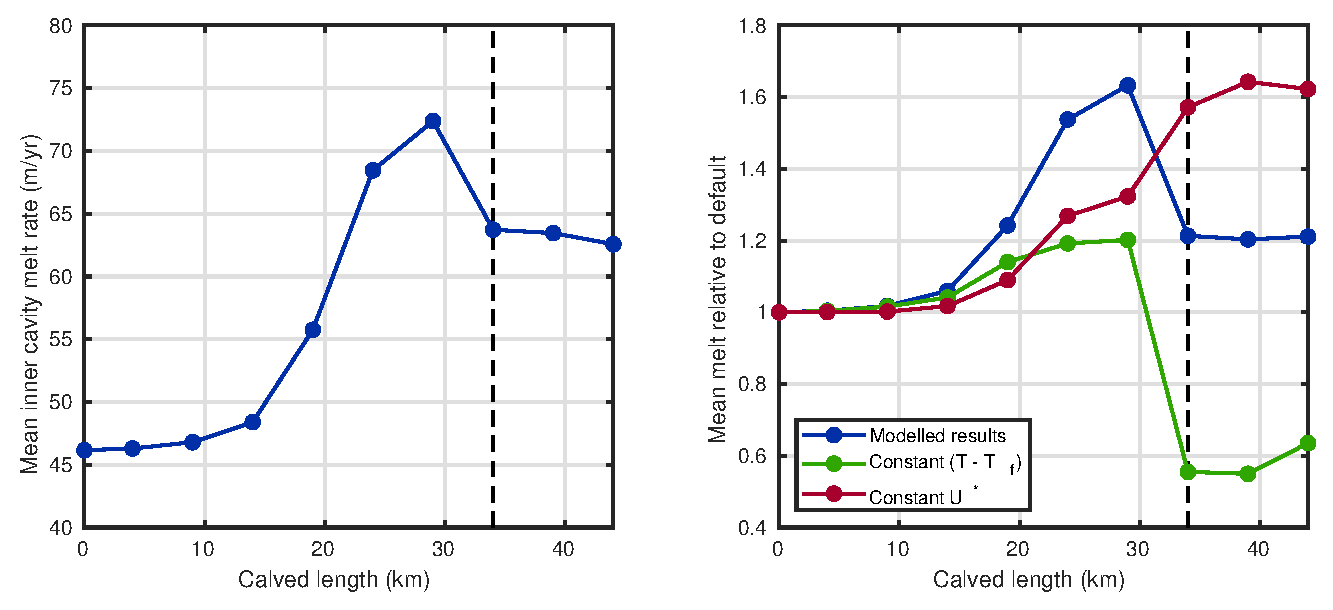
\includegraphics[width = \textwidth]{../make_figures/plots/figure4.eps}
    \caption{(a) Mean inner cavity melt rate as a function of the calved length $l_c$. The black dashed line indicates the position of the ice front when it is located directly above the seabed ridge. (b) Velocity-thermal driving decomposition: decomposition of changes in inner cavity melt rate relative to the default (uncalved) simulation into changes in boundary layer speed $U_\text{effect}$ (green curve, equation~\eqref{E:MillgateDecompU}) and thermal driving $\Delta T_{\text{effect}}$ (red curve, equation~\eqref{E:MillgateDecompDT}). The blue curve indicates the total relative change in melting (equation~\eqref{E:MillgateDecompMelt}).}
    \label{fig:figure4}
\end{figure}

%explain what the Millgate decomposition.
From equation~\eqref{E:MeltRateUdT}, we see that the melt rate is approximately proportional to the product of the boundary layer velocity and thermal driving. We investigate the relative roles of variations in boundary layer velocity and thermal driving in the changes to the inner cavity melt rate by replacing the boundary layer velocity and thermal driving fields in each of the simulations with a retreated ice front with corresponding fields from the default simulation, and calculating the resulting inner cavity melt rate, relative to the actual melt rate from that particular simulation. Explicitly, the relative effect of changes in boundary layer velocity and thermal driving on inner cavity melt rate are assessed by computing
 \begin{align}
U_{\text{effect}}(l_c) &=  \int_{\text{inner cavity}}\frac{u^*(x,y; l_c)}{u^*(x,y; l_c = 0)}, \label{E:MillgateDecompU}\\ \Delta T_{\text{effect}}(l_c) &= \int_{\text{inner cavity}}\frac{T(x,y; l_c) - T_b(x,y; l_c)}{T(x,y; l_c = 0) - T_{b}(x,y; l_c = 0)},\label{E:MillgateDecompDT}
 \end{align}
  where $u^*(x,y;l_c = 0)$ is the boundary layer velocity for the default simulation (and similarly for $T, T_b$). The quantities in~\eqref{E:MillgateDecompU}--\eqref{E:MillgateDecompDT} are compared, for a given calved length $l_c$, to the relative change in melting over the default simulation,
 \begin{equation}\label{E:MillgateDecompMelt}
   \mathcal{M}(l_c) =  \int_{\text{inner cavity}}\frac{\dot{m}(x,y)}{\dot{m}(x,y; l_c)}.
 \end{equation}
The quantities~\eqref{E:MillgateDecompU}--\eqref{E:MillgateDecompMelt} are plotted in figure~\ref{fig:figure4}b, where changes in inner cavity melt rate that result exclusively from changes in the inner cavity circulation would be indicated by indistinguishable blue and red curves, while changes in the inner cavity melt rate that result exclusively from changes in thermal driving at the ice-ocean interface would be indicated by indistinguishable blue and green curves. We refer to this comparison as a `velocity-thermal driving decomposition' henceforth. Note while the relative change in melt rate depends on the changes in velocity and thermal driving, this relationship is not linear. 

%what do these plots tell us about what is responsible for the changes?
The velocity-thermal driving decomposition for the baseline (figure~\ref{fig:figure4}b) indicates that changes in the melt rate with calving are the result of relative changes of equal magnitude in both the thermal driving and boundary layer velocity. When the ice front is located offshore of the ridge ($l_c < 25$~km), further calving results in increases in both the boundary layer velocity and thermal driving: these two effects are complimentary in the increase in melt rate with calving. When the calving front is retreated to the ridge, the thermal driving effect increases further, while velocity effect decreases sharply, indicating a significant drop in circulation in the inner cavity; this drop in circulation outweighs the more modest increase in thermal driving, leading to an overall reduction in the melt rate when front is retreated from just to offshore to directly above the ridge. 

%figure 6:  (a) row of melt rate (colours) and BSF contours, (b) zonal sections, (c,d) meridional sections
\begin{figure}
    \centering
    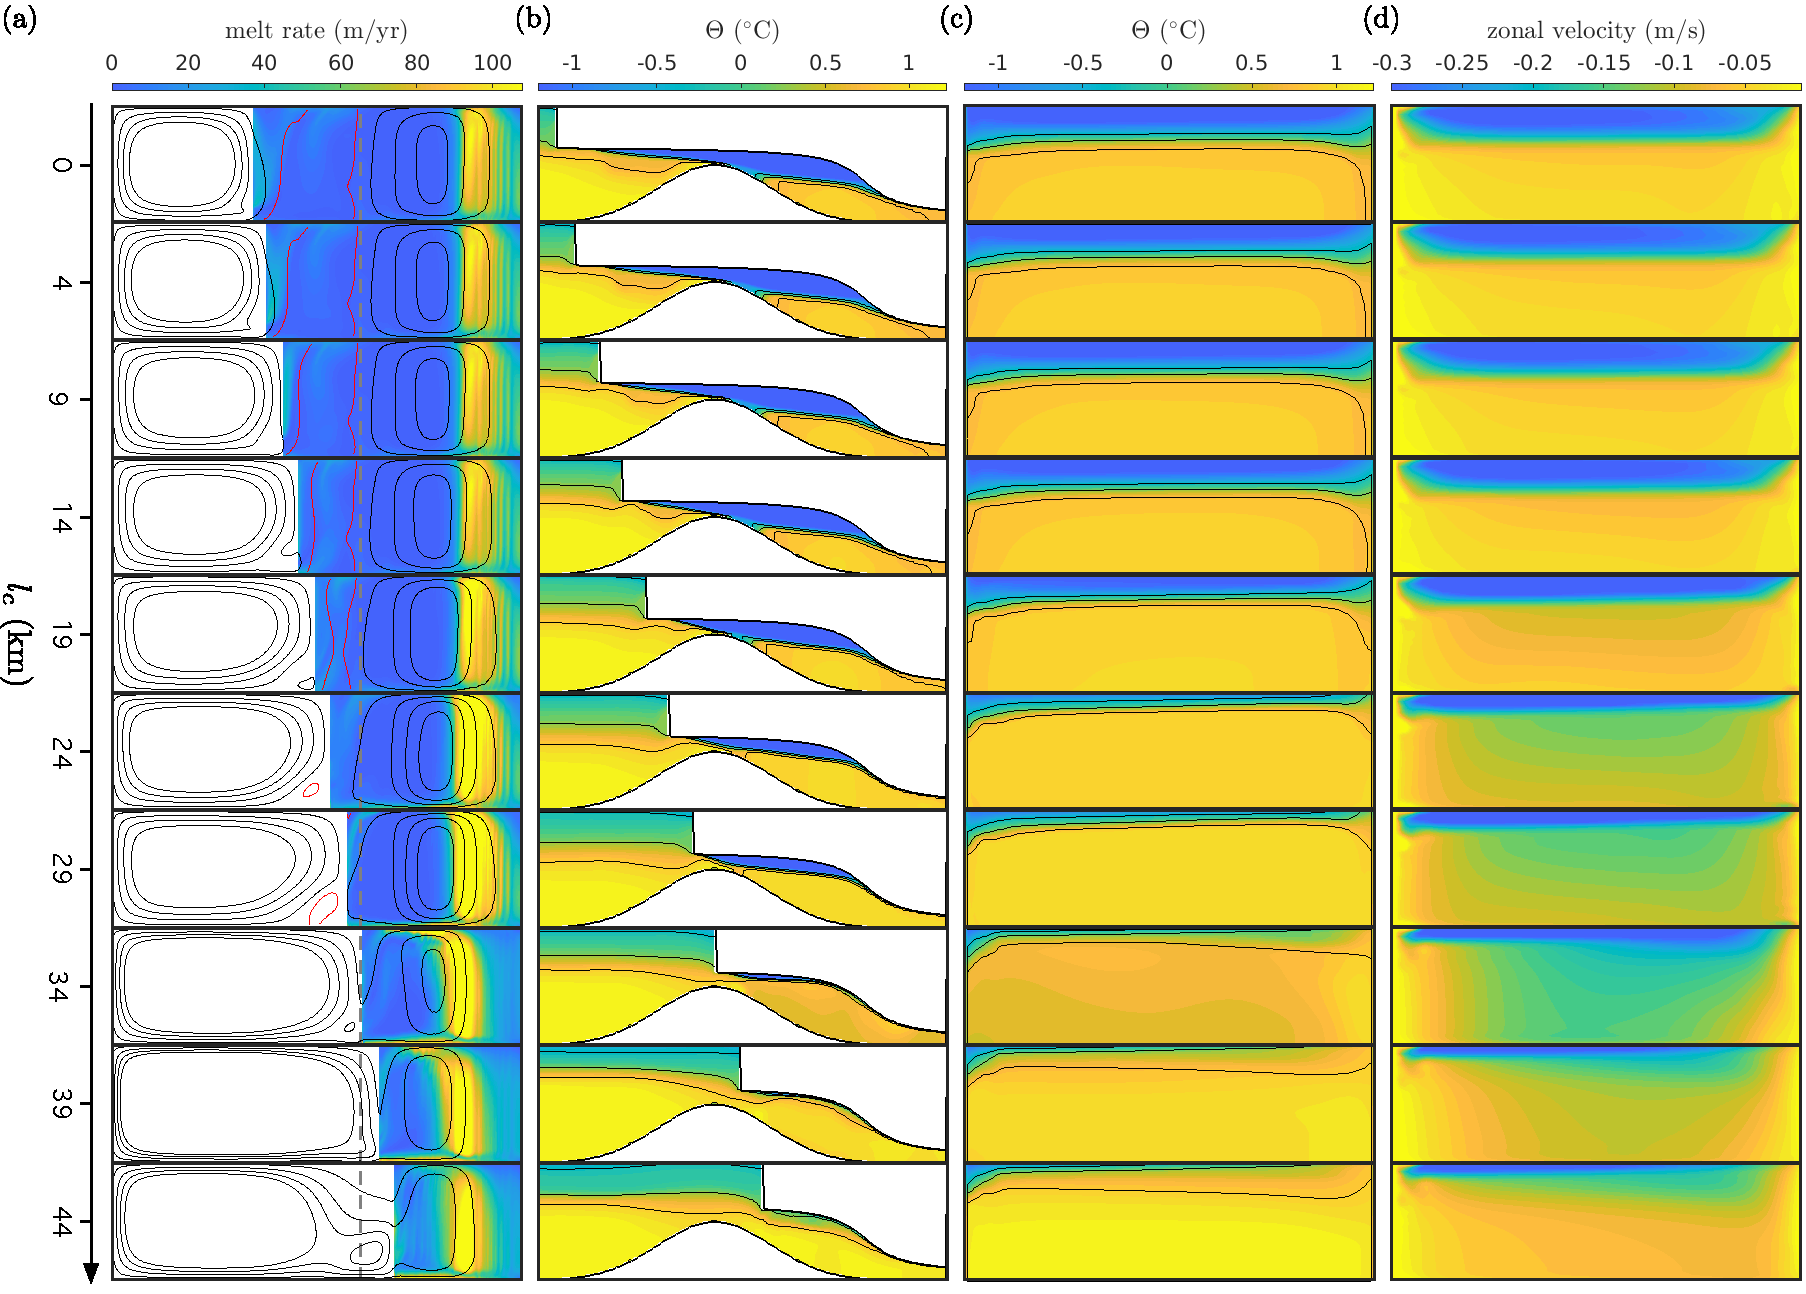
\includegraphics[width = 0.99\textwidth]{../make_figures/plots/figure5_axislabel.pdf}
    \caption{(a) Contour plots of melt rate (colours) and barotropic stream function (contours, black at levels at levels 0.1, 0.3, 0.5, and 0.7 Sv and magenta at the 0~Sv level) in the idealized simulation with $P$ = 600~m and $W$ = 100~m. The calved length $l_c$ increases from 0~km in the first row to 44~km in the final row. The empty sections indicate open ocean. (b) Contour plots of potential temperature $\Theta$ (colours) and salinity (contours, at levels 34.2, 34.4, and 34.6~psu, as in figure~\ref{fig:figure3}) taken along the centreline of the domain (magenta dashed line in figure~\ref{fig:figure3}a). White section at the top and bottom of each subplot indicate the ice shelf and seabed ridge, respectively. (c) Contour plots of potential temperature (colours) and salinity (contours, at levels 34.2, 34.4, and 34.6~psu) in the 100~m above the ridge crest (i.e. taken along the white dashed line in figure~\ref{fig:figure3}a). (d) As in (c) with colours indicating the zonal velocity.  In each case, the colour bar at the top of the column is appropriate for each plot in the column.}
    \label{fig:figure5}
\end{figure}

%how can we understand what happens.
To understand the reasons for the changes in thermal driving and boundary layer velocity, it is instructive to consider how the barotropic stream function, and zonal and meridional cross sections of temperature and velocity, change as the ice shelf calves. Plots of these quantities are shown in figure~\ref{fig:figure5} (for the default run, to which the first row corresponds, these are identical to figure~\ref{fig:figure3}b,e, and d, respectively). We focus first on the case that the ice front is located a long way ($ > 10km$) downstream of the ridge, where the situation is similar to the default case: the strong PV barrier provided by the ridge and ice draft remains in place and a topographically constrained cyclonic circulation is spun up inshore of the ridge; there is zero barotropic flow across the ridge except for at Eastern boundary (figure~\ref{fig:figure5}, first column). The Eastern wall boundary current permits warm water to reach the inner cavity, which is modified by mixing with the meltwater plume; as calving proceeds, the meltwater plume becomes marginally less prominent (figure~\ref{fig:figure5}, second column) and mixing at the Eastern boundary current is reduced slightly. Melt rates are enhanced over the baseline (figure~\ref{fig:figure4} because (a) more warm water is able to enter the inner cavity and (b) the temperature of this water is increased.

The picture remains the same as the ice front is retreated close to the ice front, except that when $l_c$ reaches, the meltwater plume detaches from the ridge crest; the hydrographic front on the north of the ridge reaches the ridge crest and some warm water is able to spill over the central portion of the ridge to the inner cavity, in addition to that entering at the eastern boundary. As a result, melt rates increase significantly (figure~\ref{fig:figure4}).

When the ice front is calved on top of the ridge ($l_c$ = 34~km), however, this picture changes in two important changes. Firstly, the strong PV barrier provided by the ridge crest and ice draft is relaxed, and the regions inshore and offshore of the ridge become more dynamically connected. The flow within the cavity is still cyclonic (figure~\ref{fig:figure5}, first column), but this circulation is far slower: the peak barotropic transport on the inner cavity is -0.86~sv for all $l_c = 29~km$, compared to -0.58 for $l_c$=34~km. The second change, is that the topographic barrier, which now consists of the ridge alone -- does not prevent warm water from spilling into the inner cavity, which become entirely flooded with warm water; although this means there is far more heat available for melting (thermal driving effect increases when calving on top of the ridge, figure~\ref{fig:figure4}b), this is outweighed by the reduced stratification and thus reduction in the velocity effect. In summary, when the calving front is receded to the top of the ridge, the two mechanisms that reduce circulation -- reductions in stratification and topographic constraint on the circulation -- outweigh the increase in heat available for melting, resulting in a significant reduction in the melt rate (figure~\ref{fig:figure4}). Further calving does not change this picture significantly, and the melt rate remains constant (figure~\ref{fig:figure4}).


\section{Effect of Cavity Geometry on Melt Response to Calving}\label{S:Results:H}
\red{Section needs second pass}
%what are we doing here and why (briefly)
In the previous section, we analyzed how, and why, the inner cavity melt rate changes with calving in the $W$=100~m case. The strength of the topographic barrier provided by the seabed ridge in combination with the ice draft was identified as a important control on the melt rate response to calving; in this section, we describe how this picture changes for larger values of $W$ ($W$ = 150~m and $W$=200~m), for which the strength of the topographic barrier is lower in the uncalved simulation.

%how do melt rates change
%In figure~\ref{fig:figure6}, we plot the inner cavity melt rate and velocity-thermal driving decomposition as a function of the calved length $l_c$ are plotted in figure for both $W$ = 150~m and $W$ = 200~m. Comparison with the corresponding results for $W$=100~m (figure~\ref{fig:figure6}a) indicates that at larger values of $H$, the inner cavity melt rate is less sensitive to calving: the range of inner cavity melt rates reduces from approximately 27\mpryr for $W$=100~m to 10\mpryr and 7\mpryr for $H$=150~m and $H$=200~m, respectively. In addition, the peak inner cavity melt rate is reached when the ice extent is greater ($l_c$ is smaller) as the gap $W$ is reduced (approximately 29~km, 14~km, and 10~km for $W$=100~m, 150~m, and 200~m, respectively).


\begin{figure}
    \centering
    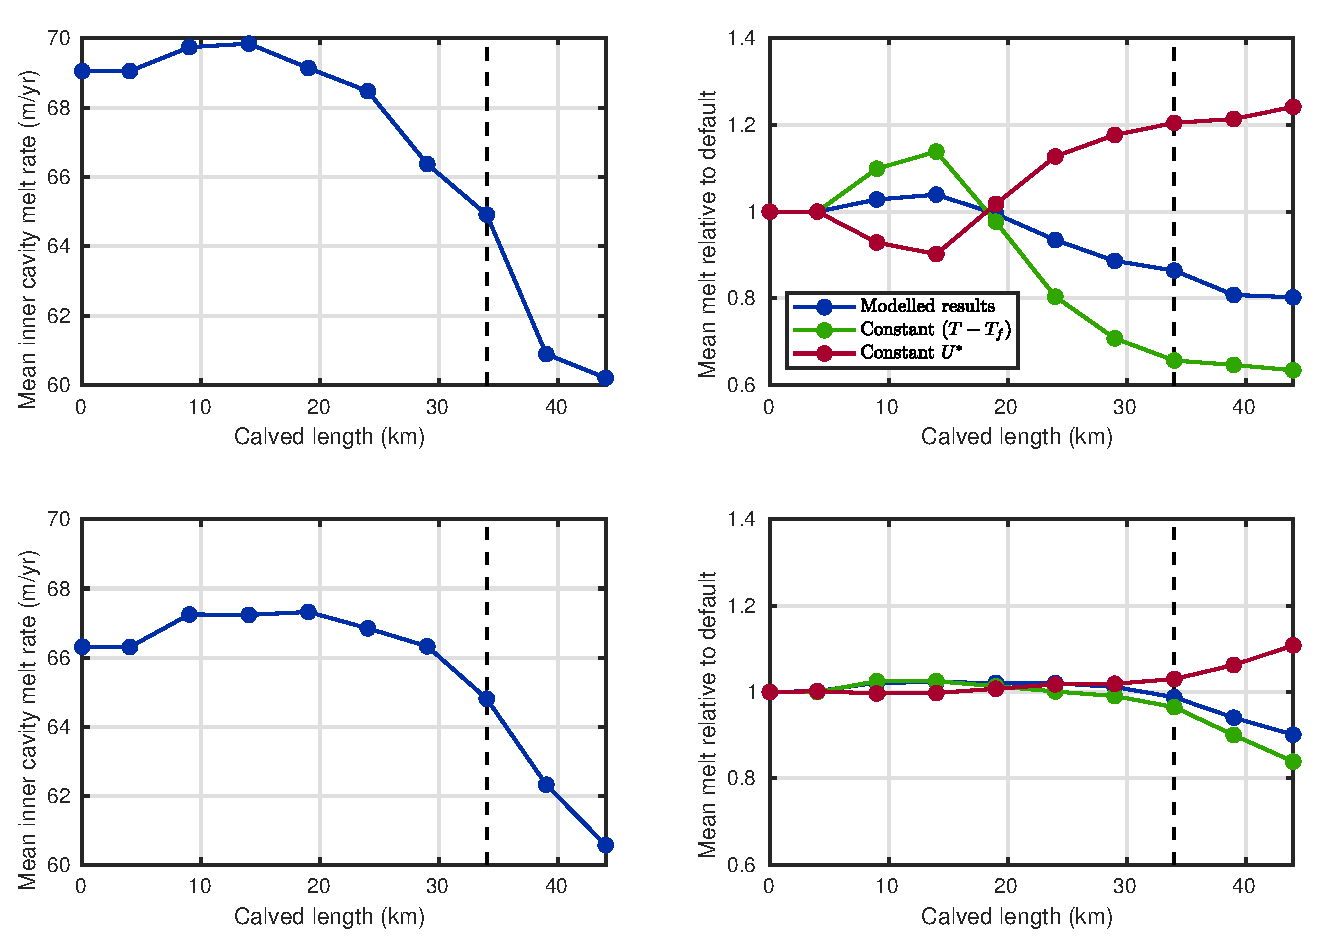
\includegraphics[width = \textwidth]{../make_figures/plots/figure6.eps}
    \caption{(a) Inner cavity melt rate as a function of the calved length $l_c$ for $W$=100~m (light grey, as in figure~\ref{fig:figure4}a), $W$=150~m (blue), and $W$=200~m (green). The black dashed line indicates the position of the ice front when it is located directly above the seabed ridge. (b)-(c) Velocity-thermal driving decomposition for (b) $W$ = 150~m and (c) $W$ = 200~m: plot of the decomposition of changes in inner cavity melt rate relative to the default (uncalved) experiment (equation~\eqref{E:MillgateDecompMelt}) into changes in boundary layer speed $U_\text{effect}$ (green curve, equation~\eqref{E:MillgateDecompU}) and thermal driving $\Delta T_{\text{effect}}$ (red curve, equation~\eqref{E:MillgateDecompDT}).}
    \label{fig:figure6}
\end{figure}

\begin{figure}
    \centering
    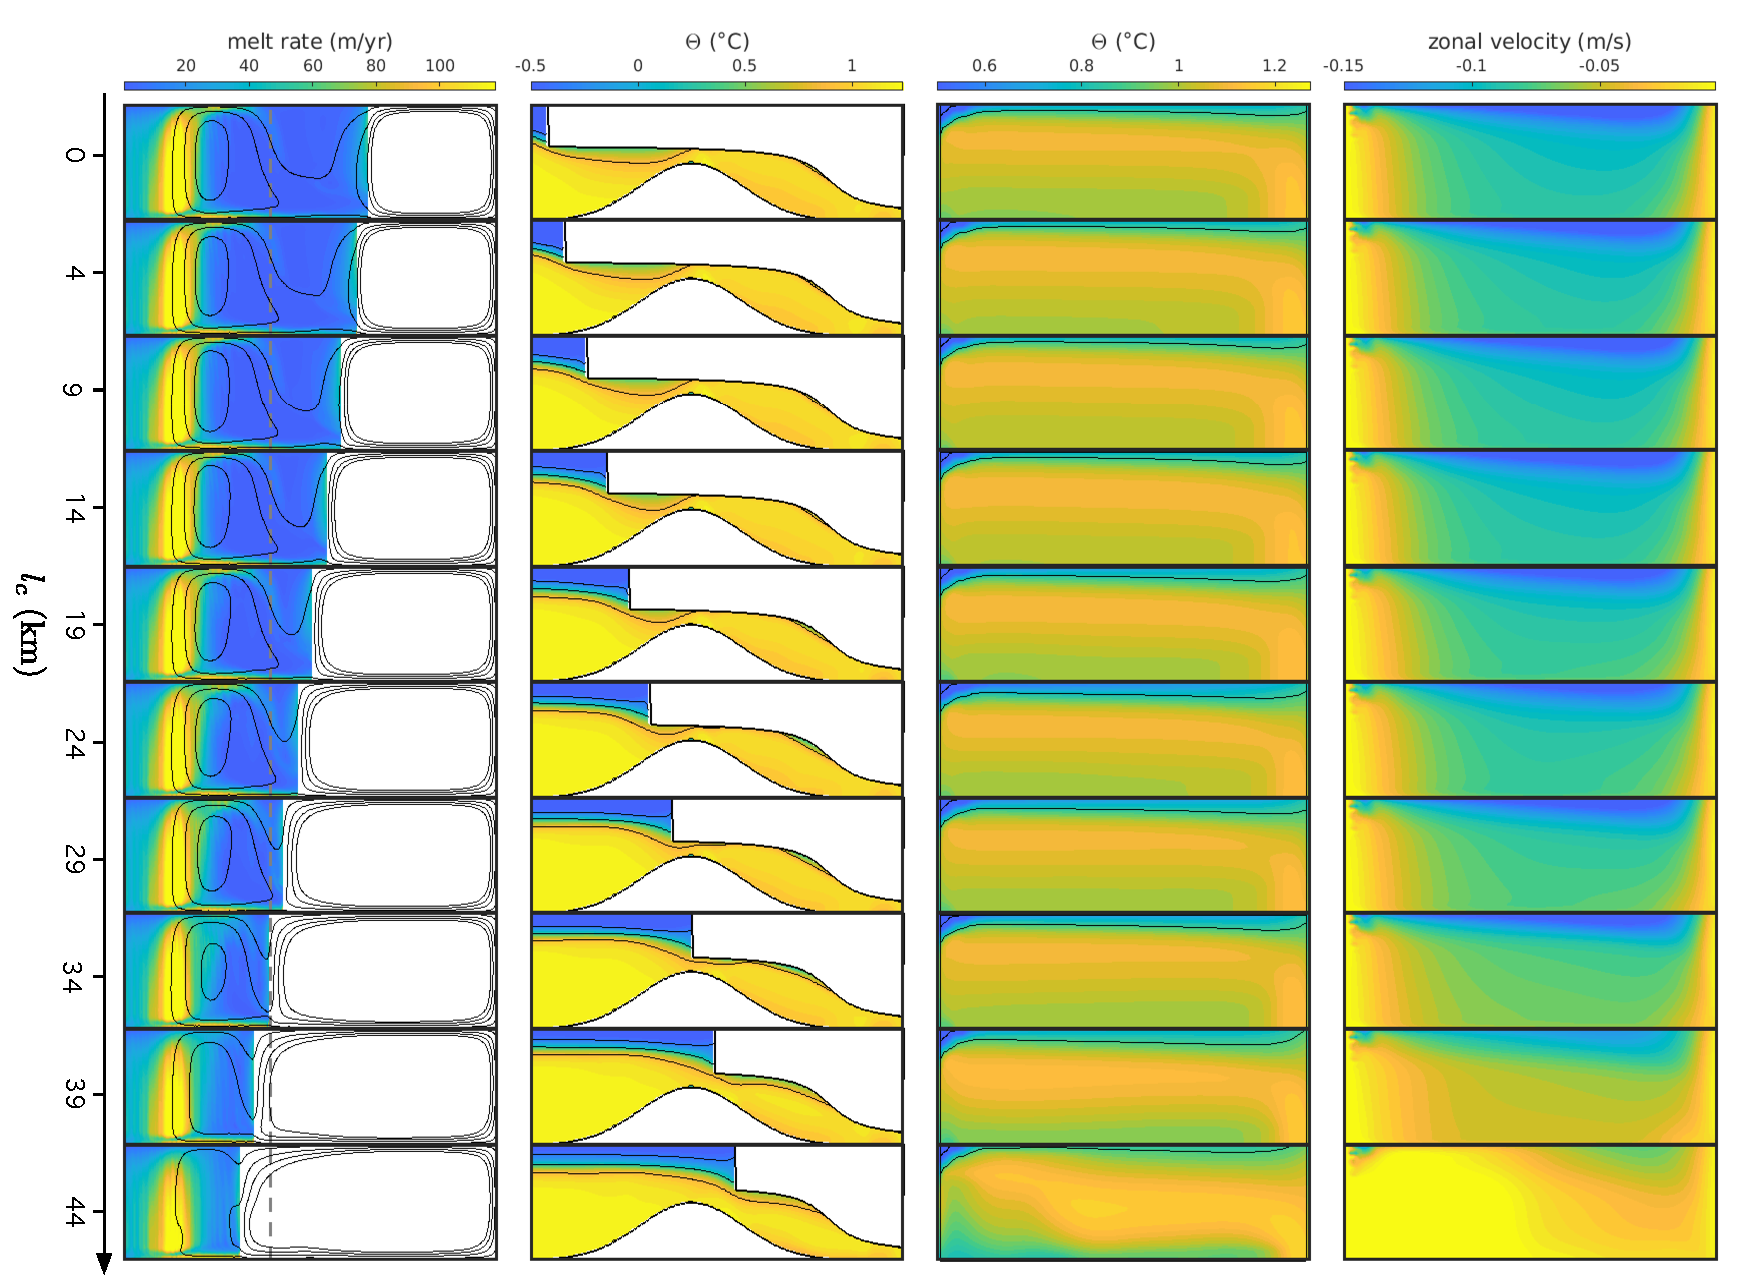
\includegraphics[width = \textwidth]{../make_figures/plots/figure7_axislabel.pdf}
    \caption{Ocean charactertistics in the idealized simulation with $P$ = 600~m and $W$ = 200~m. This plot is as in figure~\ref{fig:figure5} for the simulation with $W$=200~m. \red{needs a,b,c,d labels? Also meridional velocity I think?}}
    \label{fig:figure7}
\end{figure}


%what do we see
Mean melt rates as a function of calved length for the two larger values of $W$ ($W = 150$~m and $W = 200$~m) are plotted in figure~\ref{fig:figure6}. As in the $W = 100$ case, the inner cavity melt rate reaches a peak while the ice front is located offshore of the ridge crest. In addition, the velocity-thermal driving decomposition demonstrates that for both $W$=150~m and $W$=200~m, the reduction in inner cavity melt rates for larger $l_c$ is associated with a reduction in the inner cavity circulation that outweighs an increase in thermal driving. However, there are several important differences to the $W$=100~m case: firstly, the inner cavity melt rate is far less sensitive to calving in both the $W = 150$ and $W = 200$m cases (the difference between largest and smallest inner cavity melt rates is approximately 20\% and 10\%, respectively, compared to 60\% for $W$=100~m). Secondly, the inner cavity melt rate does not demonstrate the threshold behaviour when the calving front reaches the top of the ridge as it does in the $W$ = 100~m case.

%why do we see it
To understand these observations, it is useful to compare the cross sections in figure~\ref{fig:figure4} for $W$=100~m to those in figure~\ref{fig:figure7} for $W = 200$ case (a comparison between the $W = 100$m and $W = 150$m case is qualitatively similar to that discussed below for $W = 100$, but the differences are clearer for $W = 200$m.) In the $W$=100~m case, the two important changes were (1) relaxation of the connectivity between the inner and outer cavities and (2) greater access to the inner cavity for warm water. In the $W$=200¬m case, the inner and outer cavities are connected, even for the uncalved ($l_c$=0) simulation; there is significant transport of warm water across the ridge (figure~\ref{fig:figure7}a, c, d), not just along the and the inner cavity is almost entirely flushed with modified CDW (figure~\ref{fig:figure7}b). In other words, the inner cavity is \textit{always} saturated with warm water and their is always a strong connection between inner and outer cavities; calving does not change this, and melt rates are approximately independent of the ice front position.


%\begin{itemize}
%    \item Domains are connected even in the default run, and the inner cavity is entirely flushed with warm water. This is different to the `fully' calved $W = 100$m case because the ridge still provides a strong pv barrier constraining the flow to the inner cavity and strongly bounding it, permitting high velocities necessary to allow high mean melt rates.
%
%\end{itemize}


\section{Effect of Hydrographic Conditions on Melt Response to Calving}\label{S:Results:P}
Before moving on to assess how melt rates change with calving in realistic simulations of Pine Island, we briefly consider how the picture presented in the previous two sections changes depending on the choice of hydrographic conditions to which the ocean state is restored far from the ice shelf. As mentioned, we consider a constant ridge height and thus variability in the difference between the lower layer depth and height of the ridge -- which we expect to be the a driver of the amount of warm water that is able to spill over the ridge and into the inner cavity -- is entirely captured by the variability in the value of $P$.

\begin{figure}
    \centering
    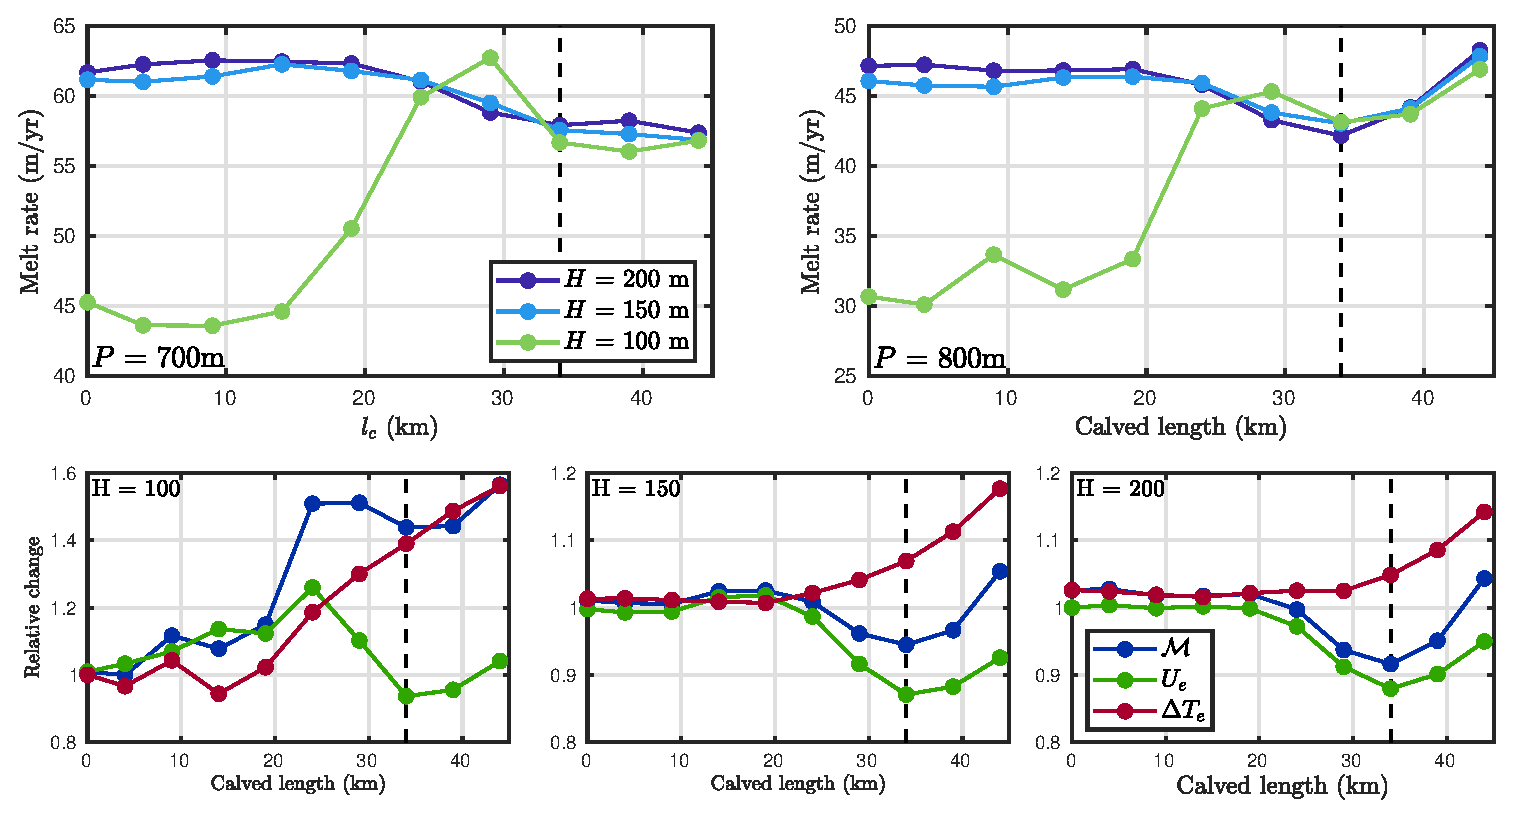
\includegraphics[width = \textwidth]{../make_figures/plots/figure8.eps}
    \caption{(a)--(b) Inner cavity melt rate as a function of calved length $l_c$ in idealized Pine Island simulations with (a) $P$=700~m and (b) $P$=800~m. Colours correspond to different values of $W$, as indicated by the legend in (a). The black dashed line indicates the location of the crest of the sea-bed ridge. (c)--(e) Velocity--thermal driving decompositions (as in figure~\ref{fig:figure4}) for the the data shown in (b): (c), (d), and (e) correspond to the results for $W$=100~m, $W$=150~, and $W$=200~m, respectively, as indicated. }
    \label{fig:figure8}
\end{figure}


% Introduce simulations with reminder of what they correspond to 
The inner cavity melt rate and velocity-thermal driving decomposition for the three experiments with $P$ = 700~m (dashed profile in figure~\ref{fig:figure2}) and the three experiments with $P$ = 800~m (dot-dashed profile in figure~\ref{fig:figure2}) are plotted in figure~\ref{fig:figure8}. The results for $P$=700~m are very similar to those for $P$=600~m, albeit with slightly lower melt rates, and can be summarized similarly: for the narrowest gap ($W$=100~m), the inner cavity melt rate is very sensitive to the front position; it increases rapidly with calving as the calving front approaches the ridge, before dropping off sharply when the ice front reaches the top of the ridge and stabilizing for further calving events. For the wider gaps ($W$=150~m, $W$=200~m), the melt rates are far less sensitive to changes in ice front position, reaching a peak when the ice front is some way upstream of the ridge (figure~\ref{fig:figure8}) and decrease steadily with further calving events. The velocity-thermal driving decompositions for the experiments with $P$=700~m (not shown) reveal that, as in the $P$=600~m case, these observations can be explained by the competition between velocity changes owing to stratification and confinement of the cyclonic, and the increased heat available for melting, in the inner cavity. The similarity between the $P$=600~m and $P$=700~m cases is perhaps unsurprising when framed in terms of the relationship between the CDW layer depth and the height of the ridge: in both of these cases, the CDW layer extends all the way to the top of the ridge (see figure~\ref{fig:figure2}) and thus the seabed ridge alone does not provide a significant barrier to CDW access to the inner cavity.

%results are different for P = 800 -- how?
In the $P = 800$ case, the melt rate increases with calving at while the ice front is located offshore of the ridge, as in the $P$=700~m and $P$=800~m cases, before reducing when the ice front is retreated to directly above the ridge, an effect that is associated with a reduction in boundary layer velocity (figure~\ref{fig:figure8}). However, unlike the $P$=700~m and $P$=600~m cases, subsequent calving events result in an increase in inner cavity melt rate that is associated with an increase in boundary layer velocity. The important difference in this case is the now, the seabed ridge alone is able to provide a significant barrier that prevents warm water from reaching the inner cavity (the CDW layer in the outer cavity does not extend to the top of the ridge), and thus the inner cavity is not entirely flushed with CDW unlike in the simulations with smaller values of $P$. Further calving events thus increase the stratification further leading to a strengthening of the circulation, that works in tandem with increased heat content to increase the inner cavity melt rate.


\begin{figure}
    \centering
    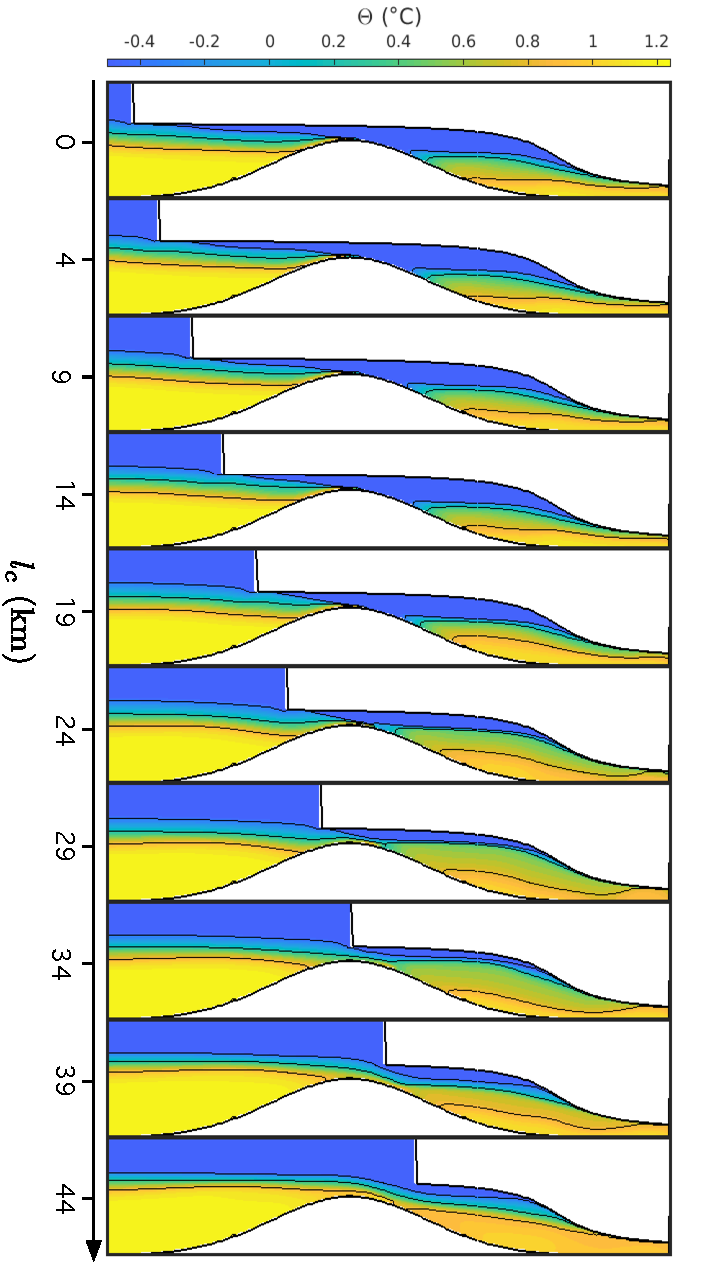
\includegraphics[width = 0.35\textwidth]{../make_figures/plots/figure9_axislabel.pdf}
    \caption{Meridional cross sections for simulations with $P$=800~m, $W$ = 100~m. This plot is as in figure~\ref{fig:figure5}b for the simulation with $P$=800~m, $W$ = 100~m.  \red{This figure will be text wrapped.} }
    \label{fig:figure9}
\end{figure}

\section{Pine Island Simulations}
% intro to the section
The idealized modelling reveals how melt rates near the grounding line are expected to respond to calving events in a cavity with a seabed ridge that is uniform in the zonal direction. These idealized simulations inform our understanding of a similar experiment in a realistic Pine Island domain. In this section, we describe this experiments, and present and analyze the results.

\begin{figure}
    \centering
    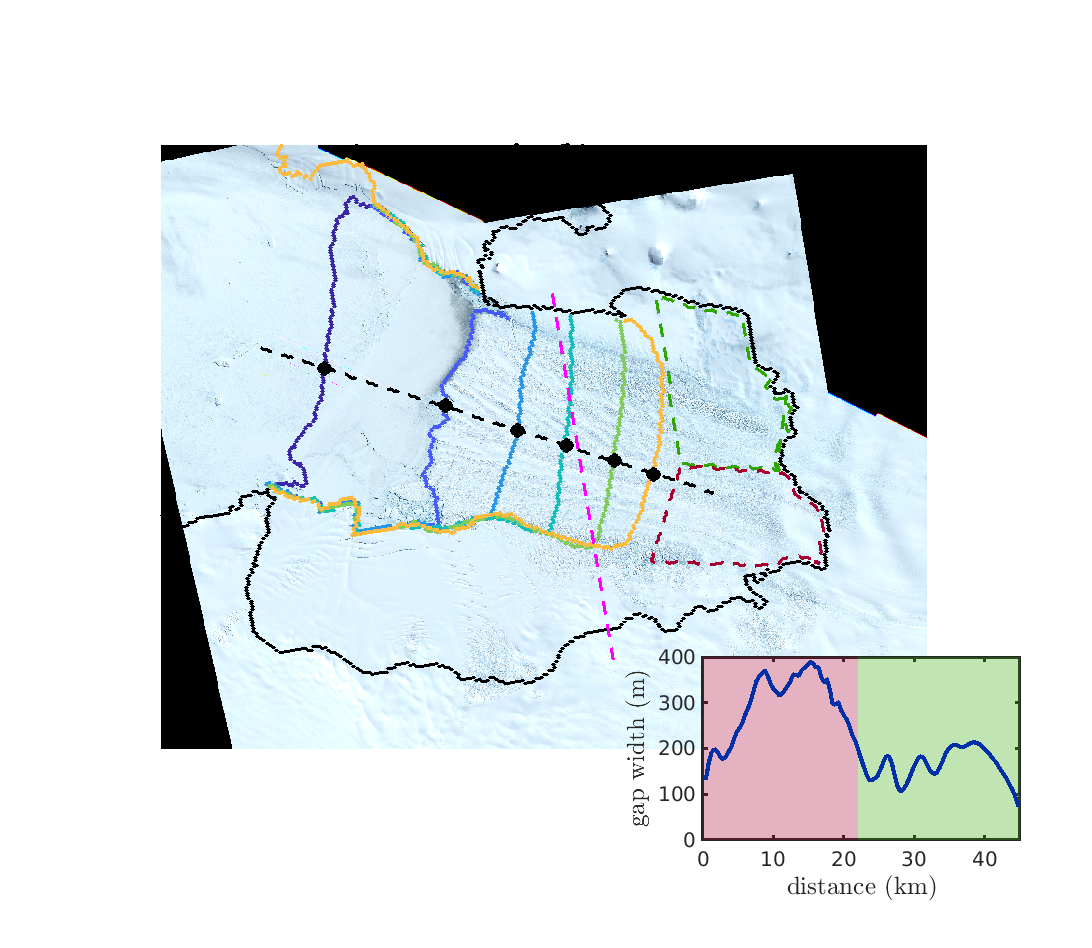
\includegraphics[width = 0.75\textwidth]{../make_figures/plots/figure10.eps}
    \caption{Ice front positions in a simulations of cavity circulation under Pine Island. Each simulation corresponds to a different ice front position, indicated by the curves in the purple to yellow colormap curves; dark purple and blue ice fronts correspond to the 2009 and 2020 front positions, respectively. The solid black line indicates the 2009 grounding line position from~\cite{Joughin2010GRL}. The blue dashed line roughly indicates the centreline of the cavity, along which the calved length is measured, and the black dashed line approximately indicates the peak of the sea bed ridge, as in figure~\ref{fig:figure1}. The cyan (North) and magenta (South) boxes indicate the inner cavity regions considered in the experiments. Inset: plot of the vertical gap between the ridge crest and the ice draft, measured along the black dashed line in the main figure. cyan and magenta shaded sections roughly correspond to locations immediately upstream of the correspondingly coloured boxes in the main figure. The background image is a Sentinel 2 mosaic from November 2020. \red{add lat/lon lines as grid?}}
    \label{fig:figure10}
\end{figure}

%Describe experiments
\subsection{Experiment Details}
To assess the effect of calving events on the sub-shelf melting in Pine Island Glacier, we resolve the cavity circulation using the same ocean model as described in \S\ref{S:Experiment:Model} with six different ice shelf topographies, whose front locations are shown in figure~\ref{fig:figure10}: the first simulation (purple ice front in figure~\ref{fig:figure10}) has an ice shelf cavity that corresponds to PIIS in 2009. The second simulation (blue ice front in figure~\ref{fig:figure10}) uses the 2009 ice shelf draft, with a section of ice removed at the front to match the observed ice front position in 2020. The four further simulations similarly use the 2009 ice shelf draft with sections of fast flowing ice removed. We stress that the ice thickness, and thus grounding line position and ice shelf draft, at existing shelf locations remains the same in each simulation: only the ice front position varies between simulations and the ice thickness is not updated.  %Consistently with the idealized simulations, we refer to the simulation with the 2009 ice front as the default run.

%how do we get cavity and draft
The sub shelf cavity is computed from the ice and seabed geometry, as described by~\citeA{Dutrieux2014Science}. Briefly, the ice shelf geometry is calculated from a 40~m-resolution digital elevation model (DEM) of the ice freeboard from 2008~\cite{Korona2009Photogrammetry}, that is adjusted with a constant medium bias from observations obtained from the Autosub underwater autonomous vehicle~\cite{Jenkins2010NatureGeo}. The DEM assumes freely floating ice throughout the shelf, which may reduce its accuracy close to the grounding line. Over the continental shelf, the seabed geometry is well known from ship echo-sounding \cite{Dutrieux2014Science}, while in the cavity it calculated from an inversion of gravimetry data and corrected point-wise using the median difference between the depth from the gravimetry inversion and the Autosub observations. 

%model notes and calibration
We consider a single hydrographic forcing, corresponding to observed 2009 conditions in Pine Island Bay (dark grey line in figure~\ref{fig:figure2}b,c), to which the ocean is restored far from the ice shelf. All model parameters are as described in \S\ref{S:Experiment:Model}, with the exception of the drag coefficient that enters into the three-equation formulation for melting; this parameter is tuned to 4.5$\times10^{-3}$ to approximately match the estimated total meltwater flux in 2009 (80 km\textsuperscript{3}/yr)~\cite{Dutrieux2014Science}). % The simulated melt rate for the `uncalved' simulation with the 2009 ice shelf geometry (figure~\ref{fig:figure11}a) is consistent with observations (not shown), displaying complex features on small scales, but characterized on larger scales as being concentrated near to the grounding line, with a peak melt rate of approximately 120~m~yr\textsuperscript{-1}.

%gap is not uniform, but sort of split. Tell the reader what the different regions are.
As mentioned in \S\ref{S:Introduction} the ridge-draft gap under PIIS is not uniform but varies from 100~m at its narrowest to 400~m at its widest, and this motivated the choice of gap thicknesses $W$ in the idealized simulations of \S2--5. The ridge-draft gap (inset in figure~\ref{fig:figure10}) can be approximately partitioned into two sections: in the Southern part of the inner cavity (magenta shading on inset of figure~\ref{fig:figure10}), the gap is relatively wide, while in the Northern part of the inner cavity (cyan shading) the gap is narrow; to facilitate inferences from our idealized results -- which include a uniform ridge-draft gap -- to be made, we evaluate changes in melting with calving in two separate regions inshore of the ridge, whose boundary corresponds to the upstream extrapolation of the boundary between the narrow and wide sections of the ridge-draft gap (see figure~\ref{fig:figure10}). 

\subsection{Results}

\begin{figure}
    \centering
    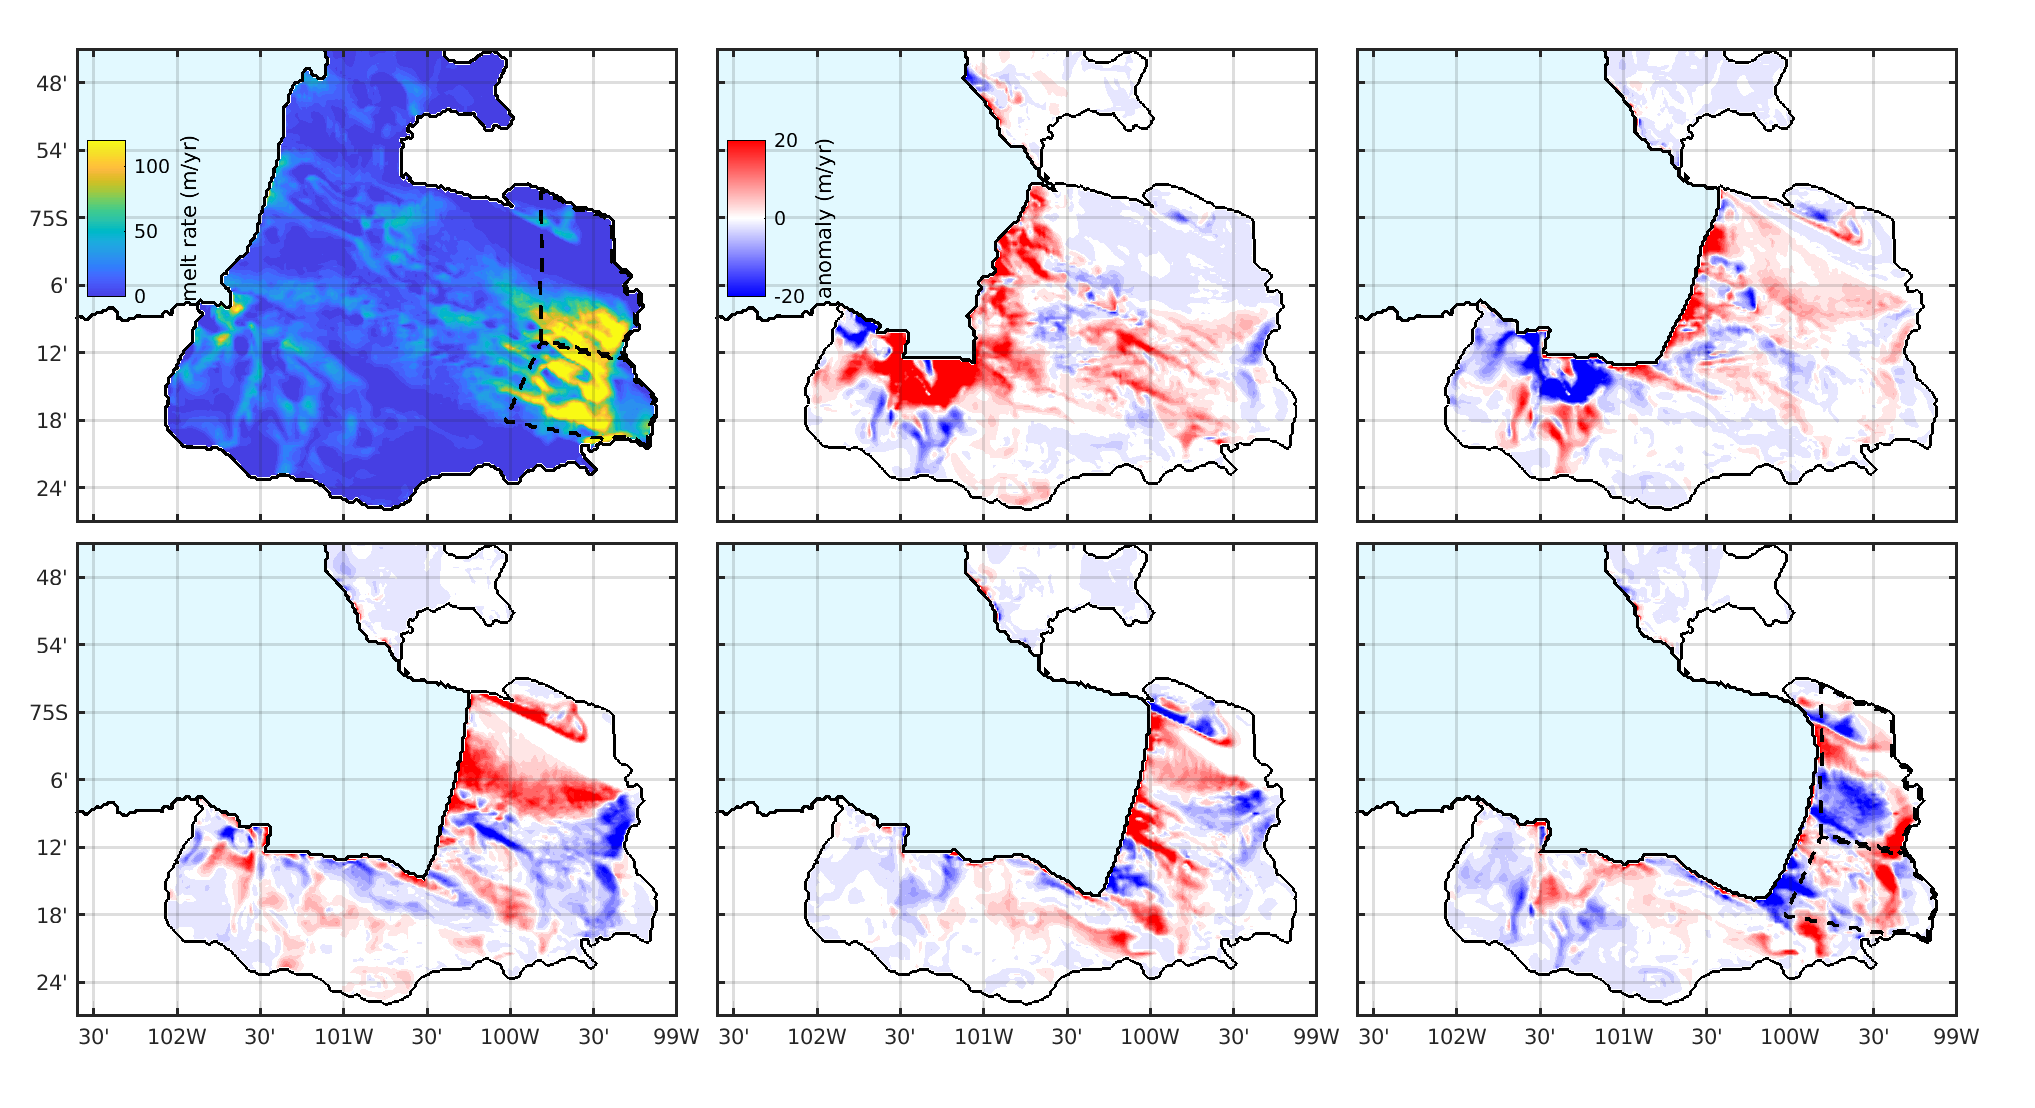
\includegraphics[width = \textwidth]{../make_figures/plots/figure11.eps}
    \caption{(a) Simulated melt rate in Pine Island with 2009 ice front. Black dashed boxes indicate the North and South boxes (see figure~\ref{fig:figure10}), where the highest melt rates are concentrated. (b)--(f) Non-cumulative melt rate anomaly in the simulations (i.e. measured relative to the previous panel). The colourbar in (b) is appropriate for each of (b)--(f). In each case, ice shelf front and grounding line (2009 grounding line position from ~\cite{Joughin2010GRL}) are shown as a solid black line. \red{Add the ridge dashed line and a scale bar here.}} 
    \label{fig:figure11}
\end{figure}


%introduce simulations
Figure~\ref{fig:figure11} contains a plot of the melt rate over the whole cavity for the default run, and the non-cumulative melt rate anomalies for the other five ice front positions. To be explicit, non-cumulative here means that red (blue, respectively) locations on these maps indicate areas in which the melt rate increases (decreases) when the ice front is retreated from the next largest configuration (i.e. changes in melt are shown relative to the previous simulation, rather than  relative to the first simulation with the 2009 front position). 

%Melt rates look qualitatively similar in the default run to the idealized case
The pattern of melt rates in the 2009 simulation (figure~\ref{fig:figure11}a) is qualitatively similar to the corresponding idealized simulation with $l_c$ = 0: peak melt rates concentrated near to the grounding line, reaching a peak of approximately 120~\mpryr several kilometers downstream of it, while the melt rate in the majority of the shelf is below 20~\mpryr.  In addition, melt rates are slightly higher on the Coriolis favoured Western boundaries, although this picture is complicated by the oblique orientation of Pine Island, and the complex geometry of both the ice shelf base and seabed. The pattern of simulated melt rates under PIIS is are consistent with observations of PIIS melting \cite{Dutrieux2014Science} and other numerical simulations of cavity circulation under PIIS \cite{Heimbach2012AnnGlac}.

%2009--now: large anomalies at the front
When the ice front is retreated from its 2009 position to its 2020 position, melt rates within 10~km of the ice front. This is attributed to high velocities associated with upwelling at the new ice shelf front as well as the formation of a gyre in the embayment in the exposed open ocean when the ice front is retreated from its 2009 to 2020 position, as has been observed in practice \red{ref}. The gyre results in a strong circulation along the ice shelf front, as it is a dynamic barrier to flow and provides a freshwater source to further enhance the flow. 

%2009-now: small changes in the inner cavity region
Melt rates in the inner cavity do not change significant, when the ice front is retreated from its 2009 position to its 2020 position: the average melt rate in the Northern and Southern boxes increase by approximately 1\mpryr and 2\mpryr respectively (figure~\ref{fig:figure12}a).

%Qualitative descriptions of melt anomalies: (a) characterized by complex patterns, (b) only see significant changes when calving beyond the ridge (large positive anomaly in the northern shear margin which might be important for stability), (d) melt rates decrease when ice front has retreated significantly (this is a lead in to the qualitative analysis of fig 12)
Melt rate anomalies in the simulations with possible future ice front positions display complex patterns of change, featuring large regions of both positive and negative anomalies (figure~\ref{fig:figure11}). There are several features important features of these patterns that we highlight here: firstly, with the exception of a large negative anomaly in the Southern shear margin, melt rates anomalies change significantly in the first 'future' snap, suggesting that PIIS currently has a reasonable `safety band' for changes in melt rate with calving: melt rates are not expected to change significantly until the ice shelf front has retreated some way ($>$10~km) from it current position. Secondly, however, melt rates around the Northern shear margin increase dramatically when the ice front is retreated to a position that sits (approximately) above the seabed ridge (figure~\ref{fig:figure11}d). This region of enhanced melt rates extends almost all the way to the grounding line.  Finally, melt rates decrease significantly over large portions of the areas of the ice shelf once the front has retreated a significant distance upstream of the ridge (figure~\ref{fig:figure11}f).

\begin{figure}
    \centering
    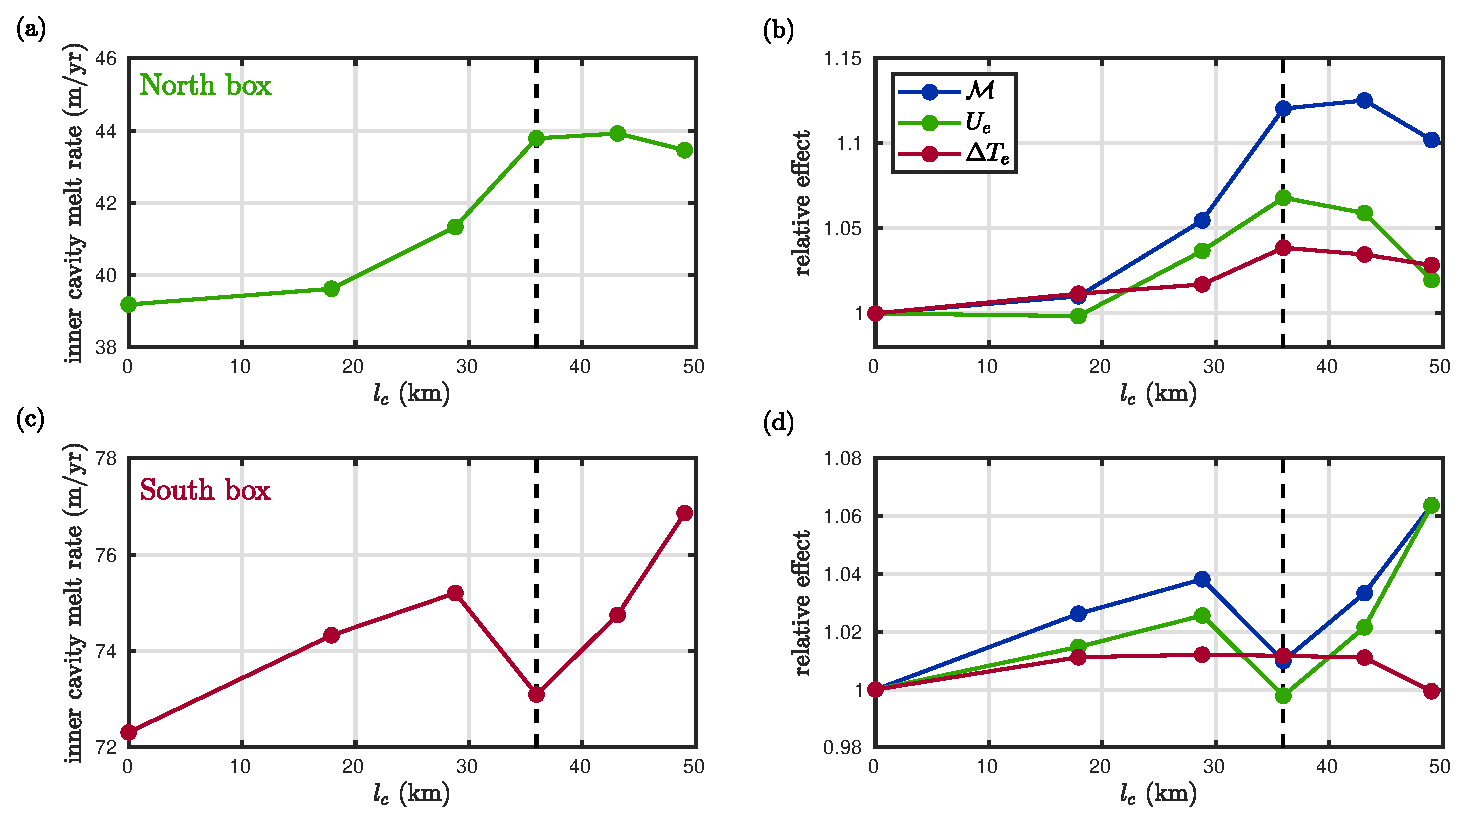
\includegraphics[width = \textwidth]{../make_figures/plots/figure12.eps}
    \caption{(a), (c) Average melt rate as a function of calved length $l_c$ in realistic simulations of Pine Island. Plots (a) and (c) correspond to the North (green dashed) and South (red dashed) boxes shown in figure~\ref{fig:figure10}, respectively. The calved length $l_c$ is the distance measured along the black dashed line in figure~\ref{fig:figure10}, taken relative to the 2009 ice front position (purple curve in figure~\ref{fig:figure10}.). (b), (d) Velocity-thermal driving decomposition for the changes in melt rate shown in (a) and (c), respectively. As indicated by the legend in (b) and (d), blue, red, and green curves correspond to simulated changes $\mathcal{M}$, velocity effects $U_e$, and thermal driving effects $\Delta T_e$, respectively. In all plots, the black dashed line approximately corresponds to the location of the peak of the ridge along the black dashed line in figure~\ref{fig:figure10}, where it intersects with the blue dashed line. \red{Perhaps label 2009 and 2020 in (a) and (c). different colours for the boxes -- distinguish them from lines in (b), (d) -- would be nice (also need to do in fig 10 if so)}}\label{fig:figure12}
\end{figure}

%these qualitative observations sort of agree with the mean melt rate plots
 These observations are in qualitative agreement with the idealized simulations presented in \S2--5. To go beyond this qualitative assessment, we plot in figure~\ref{fig:figure12}, the mean melt rate as a function of calved length. In the Northern box, mean melt rates remain approximately constant until the ice front approaches the seabed ridge, where the increase dramatically, before reducing weakly when the ice front is retreated. In the Southern box, melt rates are less variables, but may be characterized by increases while the ice front is located downstream of the seabed ridge, before dropping temporarily when the ice front is retreated to the ridge and subsequently increasing again. 
 
%northern box 'hides' behind a narrow gap -- make comparison with the narrow idealized case
Our interpretation of these results is guided by the idealized simulations presented in \S\ref{S:Baseline}--\ref{S:Results:P}. The Northern section of the inner cavity `hides behind' a relatively narrow gap between the seabed ridge and the ice draft (see inset in figure~\ref{fig:figure10}), and the change in melt rates with calving behaves in a qualitatively similar manner to idealized results with narrow ($W$=100~m, $W$=150~m) gaps, as mentioned. A velocity-thermal decomposition of these changes in melt rates indicates that -- as in the corresponding idealized case -- both enhancement in thermal driving and velocity, which are of a similar magnitude, contribute to the changes while the ice front is located downstream of the ridge, and that a reduction in the boundary layer velocity is responsible for the decrease in melt rates when calving beyond the ridge. Taking inference from the idealized simulations, the enhancement in melt rates while the ice front is located offshore of the ridge is driven by increased heat access at the margin and enhanced circulation within the inner cavity that results from the associated increase in stratification, while the reduction in melt rates when the ice front is retreated to the ridge results from a relaxation of the confinement of the cyclonic circulation in the inner cavity and associated reduction in stratification.

%In the idealized case, however, the effect of a reduction in the boundary layer velocity was stronger, and the decrease in melt rate larger, than in this realistic case; we attribute this difference to the splitting of a connected domain into two sub-regions, and the particular complexities of the realistic cavity.

%southern box 'hides' behind a wide gap -- make comparison with the wide idealized case
The Southern box `hides behind' a relatively wide gap between the seabed ridge and the ice draft. As was the case for idealized simulations with wide ($W \gtreq$200~m), the mean melt rate is far less sensitive to the ice front position in this case: the difference between the minimum and maximum melt rates in the Southern box is approximately 6\%, which is almost half of the corresponding value in the Northern box. The overall trend of increasing melt rates except for a drop when the ice front is located on top of the ridge associated with a reduction in velocities (figure~\ref{fig:figure12} --  is reminiscent of the results of the idealized simulations with a lower pycnocline (see figure~\ref{fig:figure8}(b)--(e)). Drawing analogy to the idealized cases, this suggests that the hydrography in the Southern cavity is not entirely saturated, and significant calving continues to increase stratification in this region, unlike in the Northern box, which is entirely flushed with warm water.

\section{Discussion}\label{S:Discussion}

%haven't yet seen big anomalies in melt rates at the gl --> suggests that buttressing changes driven by calving, not melting. Need coupled model to probe interaction between them
For the immediate future of PIIS, the salient observation from the realistic simulations presented in the previous section is that the inner cavity melt rates do not change significantly when the ice front is receded from its 2009 position to its 2020 position. This suggests that changes in melting associated with relaxation of the topographic barrier under PIIS have not yet occurred and thus the reduction in buttressing that resulted in the recent acceleration of PIG \cite{Joughin2021ScienceAdv} derives primarily from the geometric changes to the ice shelf, rather than melting changes that followed these calving events. On longer timescales, these two processes are coupled; investigating their relationship requires the use of a coupled-ice ocean model, which is beyond the scope of this paper. Here, we are concerned with the immediate melt response to calving, rather than the subsequent ice dynamic response. 

%use this nice lead in to talk about shortcomings from not updating the cavity thickness 
Our lack of ice dynamics considerations remains a limitation of this study, however. In particular, with the exception of the removing the appropriate section of the ice shelf, the ice shelf cavity and grounding line position remain identical between simulations: the geometry of ice shelf cavity is not updated based on the dynamical ice response to calving. In practice, the recent (2015--2020) acceleration of PIG, with increases in speed of $>$10\% over large sections of the ice shelf and grounded ice, will lead to ice shelf thinning and thus grounding line retreat, directly impacting the cavity geometry.  Further calving events that may occur, and associated loss of buttressing, will similarly encourage grounding line retreat and cavity geometry changes. 

%Despite little change in inner cavity, have a large anomaly at front
Our simulations suggest that the region close ($<$10~km) to the ice front is one area that will experience a large increase in melt rates as a result of the recent calving of PIIS. Enhanced melt rates will lead to significant local thinning, which may encourage further calving events: the critical cliff height for collapse is thought to be strongly dependent function on the height of the cliff~\cite[ for example]{Crawford2021NatureComms}). In other words, the melt response to calving of Pine Island between 2009 and 2020 may promote further calving, working alongside processes such as the damage preconditioning~\cite{Lhermitte2020PNAS} and MICI~\cite{deconto2016Nature} to encourage a collapse of the ice shelf. 

%In future melt rates generally increase in future, but changes are smaller than idealized results suggest (why?)
Very broadly, our simulations suggests that future calving will lead to enhanced melting in the Northern part of the inner cavity, and to a lesser extent, the Southern part of the inner cavity. The magnitude of changes in melting with calving were similar to what was expected from the idealized simulations for the Southern section of the cavity (i.e. very small), for which the offshore ridge-seabed gap is wide. For the Northern section of the cavity (narrow ridge-seabed gap), the magnitude of changes is smaller than our idealized simulations predict. We attribute this difference to the complexities of the ice draft and seabed in the realistic simulations, and our somewhat ad hoc splitting of the inner cavity into two subsection. In particular, the ridge height is highly anisotropic along its length; our decoupling of the cavity into two sections in a simple attempt to account for this aniostropy, but in practice the two inner cavity regions are closely connected dynamically. Further work is required to understand the role of ridge anistotropy in controlling CDW access to the inner cavity.

%We also see large anomalies in the norther shear margin, which might be worrying
The large melt rate anomalies that are seen when the calving front is retreated to the top of the ridge may have a significant impact on the future behaviour of PIG. The shear margins of PIIS play an important role in buttressing the grounded ice~\cite{Lhermitte2020PNAS}; enhanced thinning of these regions may reduce buttressing and thus increase losses from the grounded ice. If calving events maintain their pace since 2015, this situation will be realized in the mid 2020s. Again, we do not attempt to make quantitative statements on the ice dynamics response to melt induced shear-margin thinning, which requires the use of a coupled ice-ocean model.

%although melt responses are not massive there is uncertainty in the ridge-gap, which might be actual response is larger
The magnitude of changes in inner cavity melt rate are not as large in the realistic simulations as in the idealized simulations. However, there is some uncertainity in both the geometry of the seabed and the ice draft in the ridge region; the sensitivity to the ridge-draft gap (via the parameter $W$) that was identified in the idealized simulations suggest that, if, in practice, the ridge-draft gap is marginally smaller than used in our realistic simulation, the melt response to calving may change significantly. In addition, the ice draft is not static but varies dynamically;: it is possible that thicker (thinner, respectively) ice sections might be advected to the ridge crest, narrowing (widening) the ridge-sea bed gap and thus increasing (decreasing) the sensitivity of melt rates to calving.

%what do results mean for melt rate parametrizations 
The results presented in this paper have implications for melt rate parametrizations. At present, no melt rate parametrizations account for the position of the ice front in computing the melt rate~\cite{AsayDavis2017CurrClimChRep}; in this paper, we have demonstrated that the ice front position can be an important control on the melt rate applied to an ice shelf. % Although the seabed ridge under PIIS is rather unique amongst ice shelves, it is one of the fastest changing and largest contributors to current ice loss front Antarctica; accurate future projections of PIG are       and thus most commonly simulated ice shelves. Often melt rate parametrizations are used in these simulations; our results suggest that current melt rate parametrizations must be enhanced to account for the seabed ridge if they are to be trusted in projections of PIIS.

%another source of uncertainty are parameter choices in the model, but they don't affect conclusions.
Finally, we note that MITgcm has a plethora of parameter choices and numerical settings, which might have an impact on the results of the simulations. These include choices of grid resolution, which are 400~m in the horizontal, to ensure mesoscale eddies are well resolved, and 10~m in the vertical here. Simulations at higher vertical resolution (5~m) did not change the results significantly, although results were somewhat different for higher resolution (20~m); this is perhaps unsurprising because exchange over the ridge crest, which we have shown to be important in controlling the inner cavity melt rate, is expected to be highly sensitive to vertical resolution. Agreement with the higher resolution simulations (5~m) gives us confidence that simulations the simulations presented here are appropriately resolving exchange processes over the ridge crest. 

\section{Summary}\label{S:Summary}
%general overview of the question and answer
The central aim of this paper is to understand how, and why, melt rates in Pine Island might change in response to past, and potential future, calving events, which might relax the topographic barrier that currently restricts CDW access to the inner cavity. We used a combination of idealized modelling -- to identify important mechanisms responsible for changes in melting -- and realistic simulations, whose interpretation was informed by the idealized modelling.

%what did we see in the idealized simulations, and stress that they can be used as an archetype for situations in which there is a geometric barrier (e.g. if the ice shelf retreats on an overdeepened bed)
In the idealized simulations, we identified a sensitive dependence on the cavity geometry in the controlling the melt response to calving via the parameter $W$ that described the gap between the seabed ridge and the ice draft. For a narrow gap ($W \lesssim$ 150~m), (1) the melt rate increases significantly while calving with the ice front located downstream of the seabed ridge, before (2) dropping off sharply when calving events take the ice front beyond the ridge provided the pycnocline is relatively high and (3) increasing further when the pycnocline is relatively. In contrast, for wide gaps ($W \gtrsim$ 150~m), the melt rate is largely invariant to calving. We identified the (sometimes complementary, and sometimes contrasting) roles of heat access to, and stratification of, the inner cavity, and confinement of the cyclonic gyre in the inner cavity in these observations; in particular, we identified that increased heat access to the inner cavity may, paradoxically, reduce melt rates because it results in reduced stratification and thus a shut down of the cyclonic circulation. Although these idealized results are intended to inform our understanding of melt rate changes in Pine Island, they can be considered an archetype for situations in which seabed geometry obscures access to the grounding line, a situation that might be realized, for example, in ice sheet retreat over an overdeepended bed. 

%main details on the results of the realistic simulations: complex pattern of changes, large anomaly at the front from 2009-2020 might promote further calving, 
The idealized picture is complicated somewhat by the complex geometry that exists in practice, but the competing effects mentioned above appear to still be present. Owing to the isotropy in the ridge-draft gap, we split the `inner-cavity' into two sections, one of which is upstream of a section of the ridge-draft gap that is relatively narrow, and the other is upstream of a section of the ridge-draft gap that is relatively narrow. In the `narrow' section, the melt rate increases with calving while the ice front is located downstream of the ridge, before reducing with further calving beyond the ridge, while in the `wide' section, the melt rate is largely independent of calving; both of these observations are consistent with, and appear to be driven by the same competing mechanisms as, the idealized simulations. In addition, these realistic simulations suggested that large increase in melt rates at the ice front should have occurred as a result of the 2020 calving event, and that a further calving event of this magnitude will lead to a significant increase in melting in the northern shear margin, both of which which may prove important for future ice shelf stability.

The magnitude of changes in the realistic simulation were not as significant as in the idealized simulations. The scale of these changes suggests that the immediate loss of ice area, rather than longer term changes in ice thickness associated with melt rate changes, is currently, and will continue to be, the most important control on buttressing changes in response to calving in PIG. Making a quantitative comparison between the strength of these two (coupled) effects requires the use of a three-dimensional coupled ice-ocean model. However, the sensitivity to geometry in the idealized results suggests that errors in the (somewhat uncertain) ice draft and seabed bathymetry or future ice dynamic changes that reduce the ridge-draft gap, might increase the sensitivity of Pine Island to further calving.


%some concluding remarks..?


%%% Suggested section heads:
% \section{Introduction}
%
% The main text should start with an introduction. Except for short
% manuscripts (such as comments and replies), the text should be divided
% into sections, each with its own heading.

% Headings should be sentence fragments and do not begin with a
% lowercase letter or number. Examples of good headings are:

% \section{Materials and Methods}
% Here is text on Materials and Methods.
%
% \subsection{A descriptive heading about methods}
% More about Methods.
%
% \section{Data} (Or section title might be a descriptive heading about data)
%
% \section{Results} (Or section title might be a descriptive heading about the
% results)
%
% \section{Conclusions}


%Text here ===>>>


%%

%  Numbered lines in equations:
%  To add line numbers to lines in equations,
%  \begin{linenomath*}
%  \begin{equation}
%  \end{equation}
%  \end{linenomath*}



%% Enter Figures and Tables near as possible to where they are first mentioned:
%
% DO NOT USE \psfrag or \subfigure commands.
%
% Figure captions go below the figure.
% Table titles go above tables;  other caption information
%  should be placed in last line of the table, using
% \multicolumn2l{$^a$ This is a table note.}
%
%----------------
% EXAMPLE FIGURES
%
% \begin{figure}
% \includegraphics{example.png}
% \caption{caption}
% \end{figure}
%
% Giving latex a width will help it to scale the figure properly. A simple trick is to use \textwidth. Try this if large figures run off the side of the page.
% \begin{figure}
% \noindent\includegraphics[width=\textwidth]{anothersample.png}
%\caption{caption}
%\label{pngfiguresample}
%\end{figure}
%
%
% If you get an error about an unknown bounding box, try specifying the width and height of the figure with the natwidth and natheight options. This is common when trying to add a PDF figure without pdflatex.
% \begin{figure}
% \noindent\includegraphics[natwidth=800px,natheight=600px]{samplefigure.pdf}
%\caption{caption}
%\label{pdffiguresample}
%\end{figure}
%
%
% PDFLatex does not seem to be able to process EPS figures. You may want to try the epstopdf package.
%

%
% ---------------
% EXAMPLE TABLE
%
% \begin{table}
% \caption{Time of the Transition Between Phase 1 and Phase 2$^{a}$}
% \centering
% \begin{tabular}{l c}
% \hline
%  Run  & Time (min)  \\
% \hline
%   $l1$  & 260   \\
%   $l2$  & 300   \\
%   $l3$  & 340   \\
%   $h1$  & 270   \\
%   $h2$  & 250   \\
%   $h3$  & 380   \\
%   $r1$  & 370   \\
%   $r2$  & 390   \\
% \hline
% \multicolumn{2}{l}{$^{a}$Footnote text here.}
% \end{tabular}
% \end{table}

%% SIDEWAYS FIGURE and TABLE
% AGU prefers the use of {sidewaystable} over {landscapetable} as it causes fewer problems.
%
% \begin{sidewaysfigure}
% \includegraphics[width=20pc]{figsamp}
% \caption{caption here}
% \label{newfig}
% \end{sidewaysfigure}
%
%  \begin{sidewaystable}
%  \caption{Caption here}
% \label{tab:signif_gap_clos}
%  \begin{tabular}{ccc}
% one&two&three\\
% four&five&six
%  \end{tabular}
%  \end{sidewaystable}

%% If using numbered lines, please surround equations with \begin{linenomath*}...\end{linenomath*}
%\begin{linenomath*}
%\begin{equation}
%y|{f} \sim g(m, \sigma),
%\end{equation}
%\end{linenomath*}

%%% End of body of article

%%%%%%%%%%%%%%%%%%%%%%%%%%%%%%%%
%% Optional Appendix goes here
%
% The \appendix command resets counters and redefines section heads
%
% After typing \appendix
%
%\section{Here Is Appendix Title}
% will show
% A: Here Is Appendix Title
%
%\appendix
%\section{Here is a sample appendix}

%%%%%%%%%%%%%%%%%%%%%%%%%%%%%%%%%%%%%%%%%%%%%%%%%%%%%%%%%%%%%%%%
%
% Optional Glossary, Notation or Acronym section goes here:
%
%%%%%%%%%%%%%%
% Glossary is only allowed in Reviews of Geophysics
%  \begin{glossary}
%  \term{Term}
%   Term Definition here
%  \term{Term}
%   Term Definition here
%  \term{Term}
%   Term Definition here
%  \end{glossary}

%
%%%%%%%%%%%%%%
% Acronyms
%   \begin{acronyms}
%   \acro{Acronym}
%   Definition here
%   \acro{EMOS}
%   Ensemble model output statistics
%   \acro{ECMWF}
%   Centre for Medium-Range Weather Forecasts
%   \end{acronyms}

%
%%%%%%%%%%%%%%
% Notation
%   \begin{notation}
%   \notation{$a+b$} Notation Definition here
%   \notation{$e=mc^2$}
%   Equation in German-born physicist Albert Einstein's theory of special
%  relativity that showed that the increased relativistic mass ($m$) of a
%  body comes from the energy of motion of the body—that is, its kinetic
%  energy ($E$)—divided by the speed of light squared ($c^2$).
%   \end{notation}




%%%%%%%%%%%%%%%%%%%%%%%%%%%%%%%%%%%%%%%%%%%%%%%%%%%%%%%%%%%%%%%%
%
%  ACKNOWLEDGMENTS
%
% The acknowledgments must list:
%
% >>>>	A statement that indicates to the reader where the data
% 	supporting the conclusions can be obtained (for example, in the
% 	references, tables, supporting information, and other databases).
%
% 	All funding sources related to this work from all authors
%
% 	Any real or perceived financial conflicts of interests for any
%	author
%
% 	Other affiliations for any author that may be perceived as
% 	having a conflict of interest with respect to the results of this
% 	paper.
%
%
% It is also the appropriate place to thank colleagues and other contributors.
% AGU does not normally allow dedications.


\acknowledgments
Enter acknowledgments, including your data availability statement, here.


%% ------------------------------------------------------------------------ %%
%% References and Citations

%%%%%%%%%%%%%%%%%%%%%%%%%%%%%%%%%%%%%%%%%%%%%%%
%
% \bibliography{<name of your .bib file>} don't specify the file extension
%
% don't specify bibliographystyle
%%%%%%%%%%%%%%%%%%%%%%%%%%%%%%%%%%%%%%%%%%%%%%%

\bibliography{mybib}



%Reference citation instructions and examples:
%
% Please use ONLY \cite and \citeA for reference citations.
% \cite for parenthetical references
% ...as shown in recent studies (Simpson et al., 2019)
% \citeA for in-text citations
% ...Simpson et al. (2019) have shown...
%
%
%...as shown by \citeA{jskilby}.
%...as shown by \citeA{lewin76}, \citeA{carson86}, \citeA{bartoldy02}, and \citeA{rinaldi03}.
%...has been shown \cite{jskilbye}.
%...has been shown \cite{lewin76,carson86,bartoldy02,rinaldi03}.
%... \cite <i.e.>[]{lewin76,carson86,bartoldy02,rinaldi03}.
%...has been shown by \cite <e.g.,>[and others]{lewin76}.
%
% apacite uses < > for prenotes and [ ] for postnotes
% DO NOT use other cite commands (e.g., \citet, \citep, \citeyear, \nocite, \citealp, etc.).
%



\end{document}



More Information and Advice:

%% ------------------------------------------------------------------------ %%
%
%  SECTION HEADS
%
%% ------------------------------------------------------------------------ %%

% Capitalize the first letter of each word (except for
% prepositions, conjunctions, and articles that are
% three or fewer letters).

% AGU follows standard outline style; therefore, there cannot be a section 1 without
% a section 2, or a section 2.3.1 without a section 2.3.2.
% Please make sure your section numbers are balanced.
% ---------------
% Level 1 head
%
% Use the \section{} command to identify level 1 heads;
% type the appropriate head wording between the curly
% brackets, as shown below.
%
%An example:
%\section{Level 1 Head: Introduction}
%
% ---------------
% Level 2 head
%
% Use the \subsection{} command to identify level 2 heads.
%An example:
%\subsection{Level 2 Head}
%
% ---------------
% Level 3 head
%
% Use the \subsubsection{} command to identify level 3 heads
%An example:
%\subsubsection{Level 3 Head}
%
%---------------
% Level 4 head
%
% Use the \subsubsubsection{} command to identify level 3 heads
% An example:
%\subsubsubsection{Level 4 Head} An example.
%
%% ------------------------------------------------------------------------ %%
%
%  IN-TEXT LISTS
%
%% ------------------------------------------------------------------------ %%
%
% Do not use bulleted lists; enumerated lists are okay.
% \begin{enumerate}
% \item
% \item
% \item
% \end{enumerate}
%
%% ------------------------------------------------------------------------ %%
%
%  EQUATIONS
%
%% ------------------------------------------------------------------------ %%

% Single-line equations are centered.
% Equation arrays will appear left-aligned.

Math coded inside display math mode \[ ...\]
 will not be numbered, e.g.,:
 \[ x^2=y^2 + z^2\]

 Math coded inside \begin{equation} and \end{equation} will
 be automatically numbered, e.g.,:
 \begin{equation}
 x^2=y^2 + z^2
 \end{equation}


% To create multiline equations, use the
% \begin{eqnarray} and \end{eqnarray} environment
% as demonstrated below.
\begin{eqnarray}
  x_{1} & = & (x - x_{0}) \cos \Theta \nonumber \\
        && + (y - y_{0}) \sin \Theta  \nonumber \\
  y_{1} & = & -(x - x_{0}) \sin \Theta \nonumber \\
        && + (y - y_{0}) \cos \Theta.
\end{eqnarray}

%If you don't want an equation number, use the star form:
%\begin{eqnarray*}...\end{eqnarray*}

% Break each line at a sign of operation
% (+, -, etc.) if possible, with the sign of operation
% on the new line.

% Indent second and subsequent lines to align with
% the first character following the equal sign on the
% first line.

% Use an \hspace{} command to insert horizontal space
% into your equation if necessary. Place an appropriate
% unit of measure between the curly braces, e.g.
% \hspace{1in}; you may have to experiment to achieve
% the correct amount of space.


%% ------------------------------------------------------------------------ %%
%
%  EQUATION NUMBERING: COUNTER
%
%% ------------------------------------------------------------------------ %%

% You may change equation numbering by resetting
% the equation counter or by explicitly numbering
% an equation.

% To explicitly number an equation, type \eqnum{}
% (with the desired number between the brackets)
% after the \begin{equation} or \begin{eqnarray}
% command.  The \eqnum{} command will affect only
% the equation it appears with; LaTeX will number
% any equations appearing later in the manuscript
% according to the equation counter.
%

% If you have a multiline equation that needs only
% one equation number, use a \nonumber command in
% front of the double backslashes (\\) as shown in
% the multiline equation above.

% If you are using line numbers, remember to surround
% equations with \begin{linenomath*}...\end{linenomath*}

%  To add line numbers to lines in equations:
%  \begin{linenomath*}
%  \begin{equation}
%  \end{equation}
%  \end{linenomath*}



